%=========================================================================
%
% Copyright 1999-2012, Owners retain copyrights to their respective works.
%
% This file is part of lb3d.
%
% lb3d is free software: you can redistribute it and/or modify it under
% the terms of the GNU Lesser General Public License as published by
% the Free Software Foundation, either version 3 of the License, or (at
% your option) any later version.
%
% lb3d is distributed in the hope that it will be useful, but WITHOUT
% ANY WARRANTY; without even the implied warranty of MERCHANTABILITY or
% FITNESS FOR A PARTICULAR PURPOSE. See the GNU Lesser General Public
% License for more details.
%
% You should have received a copy of the GNU Lesser General Public
% License along with lb3d. If not, see <http://www.gnu.org/licenses/>.
%
%=========================================================================


\documentclass[a4paper]{article}
\usepackage{texdraw}
\usepackage{graphicx}
\usepackage{xcolor}
\usepackage{amsbsy,amssymb,amsmath}
\usepackage{epsf}
\usepackage{longtable}

  \oddsidemargin=0.5truecm
  \topmargin=-1cm
  \textwidth=15cm
  \leftmargin=0cm
  \textheight=23cm

\graphicspath{{figures/}}

\begin{document}
\newcommand{\ftrue}{{\tt .true. }}
\newcommand{\ffalse}{{\tt .false. }}
\newcommand{\vect}[1]{\ensuremath{ {\bf #1  }}} 
\newcommand{\uvect}[1]{\ensuremath{ \hat{\bf #1  }} }
\newcommand{\maintainer}{Jens Harting, {\tt lb3d.phys\_at\_tue.nl}}
\newcommand{\bfx}{{\bf x}}

% Insert nifty TeXdraw macrology here.
\input txdtools

% Draw a box of given width and height, whose top is centered at
% the current graphics position.
% Return to the first graphics position.

\newcommand{\cbox}[2]{
	\realdiv #1 2 \xdiff \rlvec({\xdiff} 0)
	\rlvec(0 -#2) \rlvec(-#1 0) \rlvec(0 #2)
	\rlvec({\xdiff} 0)
}

% Do the same, but put centred text in there too.
% Note that the given width and height are doubled.

\newcommand{\ctbox}[3]{

	\rlvec(#1 0)
	\rlvec(0 -#2) \rlvec(0 -#2)
	\rlvec(-#1 0) \rlvec(-#1 0)
	\rlvec(0 #2) \rlvec(0 #2)
	\rlvec(#1 0)

	\rmove(0 -#2) \textref h:C v:C \htext{#3}
	\rmove(0 #2) % Return to the top centre.
}

% The same, but two lines of text.

\newcommand{\cdtbox}[4]{

	\rlvec(#1 0)
	\rlvec(0 -#2) \rlvec(0 -#2) \rlvec(0 -#2) \rlvec(0 -#2)
	\rlvec(-#1 0) \rlvec(-#1 0)
	\rlvec(0 #2) \rlvec(0 #2) \rlvec(0 #2) \rlvec(0 #2)
	\rlvec(#1 0)

	\rmove(0 -#2) \textref h:C v:C \htext{#3}
	\rmove(0 -#2) \textref h:C v:C \rmove(0 -0.2) \htext{#4} \rmove(0 0.2)
	\rmove(0 #2)
	\rmove(0 #2) % Return to the top centre.
}

% Macro to make two boxes,  one on top of another, connected by a vertical
% arrow, containing text.
% Return with the current position being at the bottom of the lower box.

\newcommand{\doublebox}[4]{

	\ctbox{#1}{#2}{#3}
	\rmove(0 -#2) \rmove(0 -#2) \ravec(0 -1)
	\ctbox{#1}{#2}{#4}
	\rmove(0 -#2) \rmove(0 -#2) 
}

% Macro to make three boxes,  one on top of another, connected by a vertical
% arrow, containing text.
% Return with the current position being at the bottom of the lower box.

\newcommand{\triplebox}[5]{

	\ctbox{#1}{#2}{#3}
	\rmove(0 -#2) \rmove(0 -#2) \ravec(0 -1)
	\ctbox{#1}{#2}{#4}
	\rmove(0 -#2) \rmove(0 -#2) \ravec(0 -1)
	\ctbox{#1}{#2}{#5}
	\rmove(0 -#2) \rmove(0 -#2)

}

% End TeXdraw macrology.

% Reset paragraph indentation
\setlength{\parindent}{0pt}

\thispagestyle{empty}
\flushleft
{\Huge \bf \sf
LB3D V7}\\
{\Large \sf
A Parallel Implementation of the Lattice-Boltzmann Method for Simulation of Interacting Amphiphilic Fluids\\~\\}
\normalsize

{\sf \noindent %=========================================================================
%
% Copyright 1999-2012, Owners retain copyrights to their respective works.
%
% This file is part of lb3d.
%
% lb3d is free software: you can redistribute it and/or modify it under
% the terms of the GNU Lesser General Public License as published by
% the Free Software Foundation, either version 3 of the License, or (at
% your option) any later version.
%
% lb3d is distributed in the hope that it will be useful, but WITHOUT
% ANY WARRANTY; without even the implied warranty of MERCHANTABILITY or
% FITNESS FOR A PARTICULAR PURPOSE. See the GNU Lesser General Public
% License for more details.
%
% You should have received a copy of the GNU Lesser General Public
% License along with lb3d. If not, see <http://www.gnu.org/licenses/>.
%
%=========================================================================

E.~Breitmoser,
J.~Chin, 
C.~Dan,
F.~D\"orfler,
S.~Frijters,
G.~Giupponi,
N.~Gonz\'{a}lez-Segredo, 
F.~G\"unther,
J.~Harting, 
M.~Harvey,
M.~Hecht,
S.~Jha,
F.~Janoschek,
F.~Jansen,
C.~Kunert,
M.~Lujan,
I.~Murray,
A.~Narv\'aez,
M.~Nekovee, 
A.~Porter,
F.~Raischel,
R.~Saksena,
S.~Schmieschek,
D.~Sinz,
M.~Venturoli, 
T.~Zauner
\\}


\vfill
\begin{center}
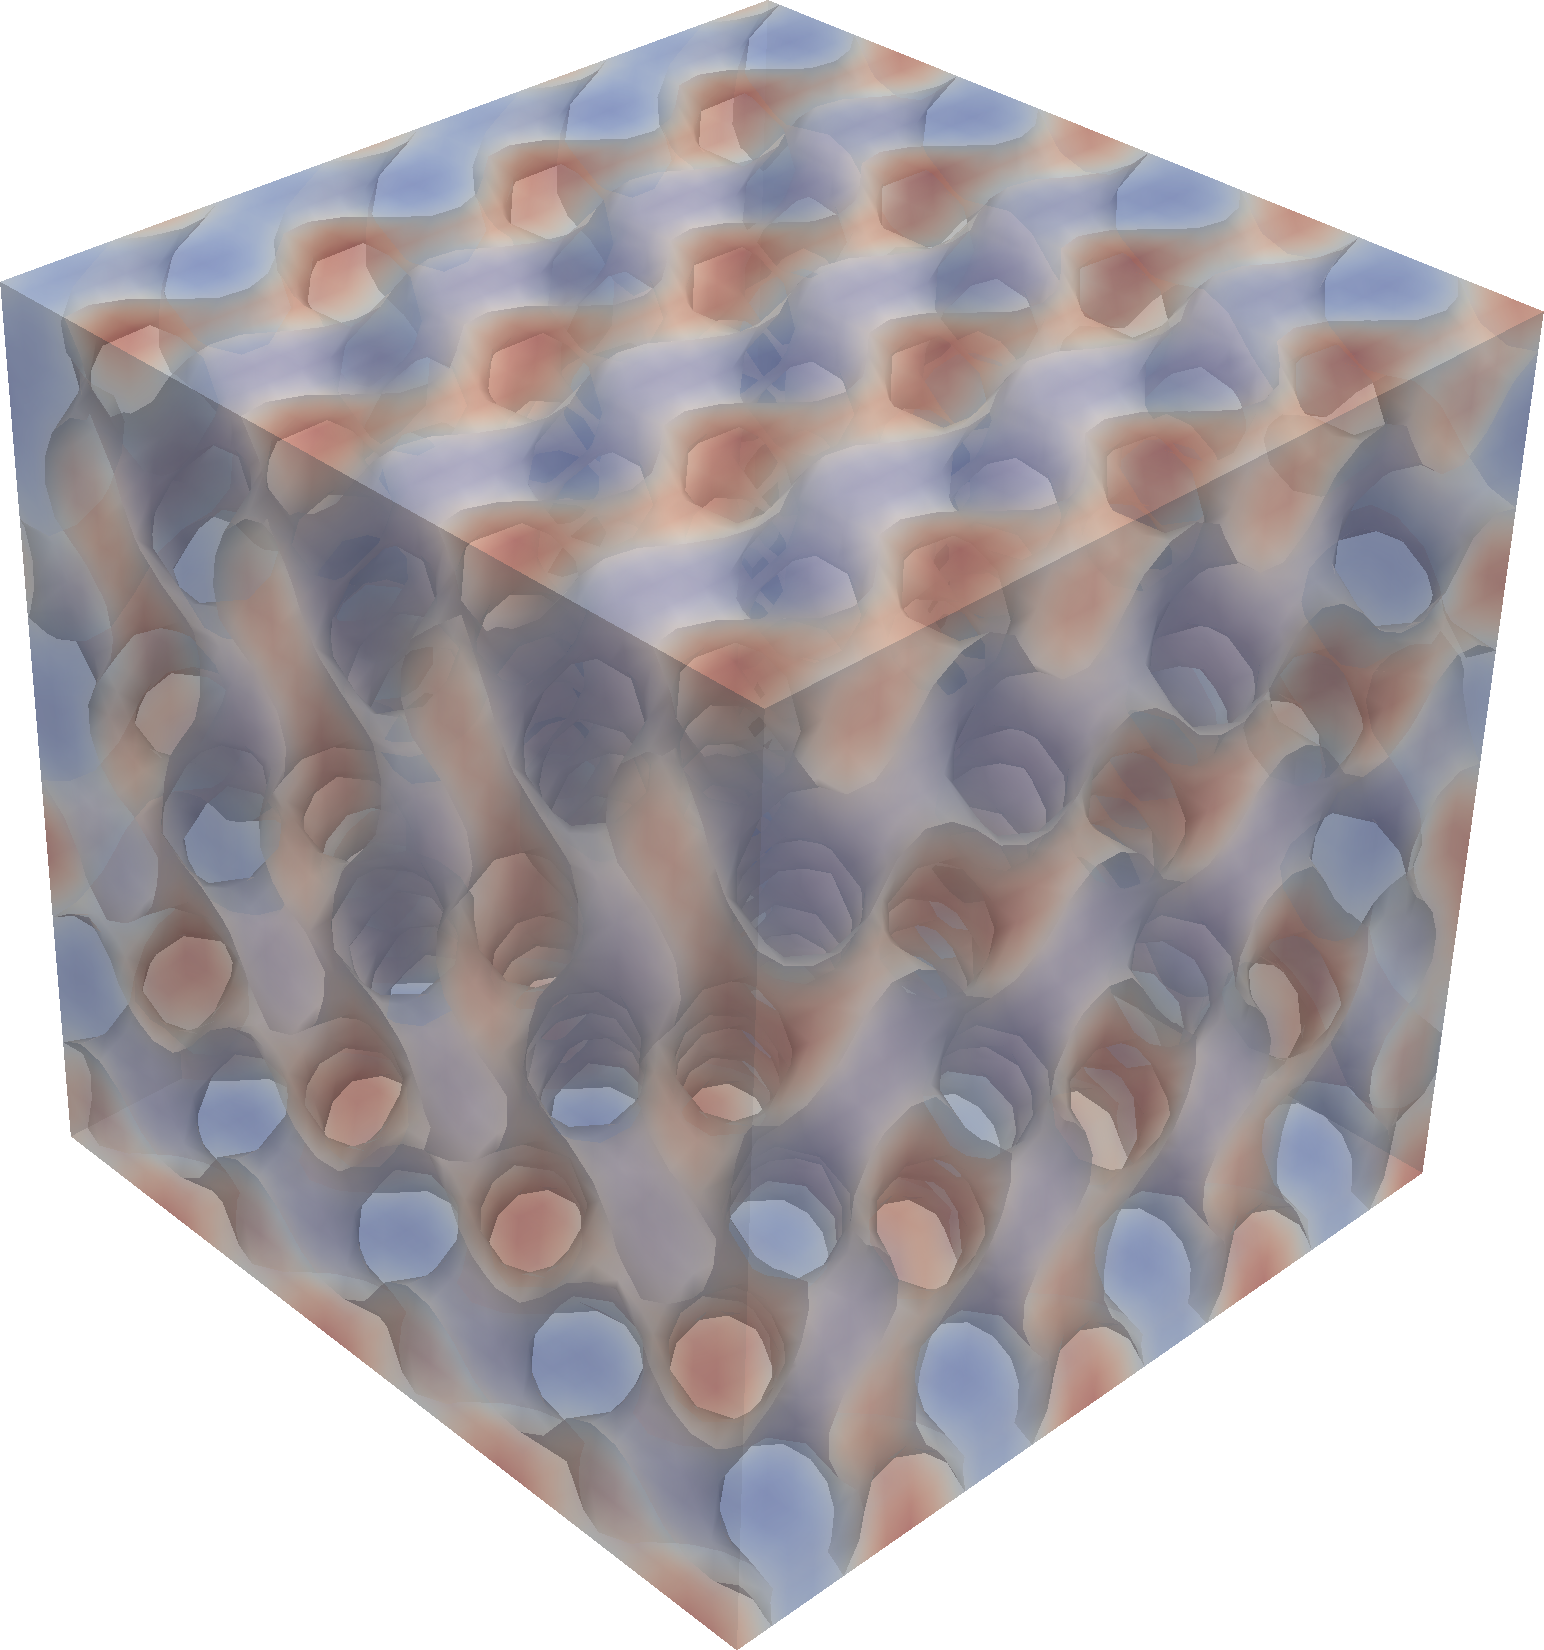
\includegraphics[width=0.8\textwidth]{gyroid.png}
\end{center}
\vfill
\newpage
~
\vfill
\section*{License disclosure}
\addcontentsline{toc}{section}{License disclosure}
Copyright 1999-2012, Owners retain copyrights to their respective works.\\~\\

This manual is part of LB3D.\\~\\

LB3D is free software: you can redistribute it and/or modify it under the terms of the GNU Lesser General Public License as published by the Free Software Foundation, either version 3 of the License, or (at your option) any later version.

LB3D is distributed in the hope that it will be useful, but WITHOUT ANY WARRANTY; without even the implied warranty of MERCHANTABILITY or FITNESS FOR A PARTICULAR PURPOSE. See the GNU Lesser General Public License for more details.

You should have received a copy of the GNU Lesser General Public License along with LB3D. If not, see \textless http://www.gnu.org/licenses/\textgreater.
\newpage

\tableofcontents
\newpage

\section{Introduction}
  
This document describes a parallel-processing implementation of our
Lattice-Boltzmann (LB) model for amphiphilic fluid dynamics
\cite{bib:maziar1,bib:maziar2}.  The main features of the model, which
distinguish it from prior lattice-Boltzmann schemes are 

\begin{itemize}
\item 
The model conserves mass separately for each chemical species present (water,
oil, amphiphile) and maintains a vector-valued orientational degree of freedom
for the amphiphilic species. 
\item
It offers  control of the viscosities of each component separately (by
adjusting the corresponding relaxation time parameter) and molecular masses of
the various species present.
\item
Interactions between fluid components are incorporated from bottom-up
by introducing self-consistently generated mean-field
forces between the fluid particles, 
rather than by a-priori positing a macroscopic free energy functional.
\end{itemize}
With the amphiphilic interactions extinguished the current version 
of the model reduces to 
the Shan-Chen Lattice-Boltzmann model \cite{bib:shan-chen} 
for binary immiscible fluids.
For a detailed description of the model and its  lattice-Boltzmann and
lattice-gas automata (LGA) predecessor
we refer the reader to 
\cite{bib:bce,bib:shan-chen,bib:maziar1,bib:maziar2}.

This document gives a brief overview of the algorithms involved,
instructions for how to compile and run the code on different 
parallel platforms, a detailed description of input and output,
as well as visualization of data and parallel performance of the code.

\section{Overview of the program}
The core of the code is a Lattice-Boltzmann solver, written for use on
multi-CPU architectures.  The parallel codes are written in standard FORTRAN90,
and make use of a number of features of that language that are object-oriented
in spirit.  The codes utilize the standard message passing MPI for
synchronization and communication between processors.  The code can be used in
Single Data Multiple Processors (SDMP) mode, where the load of one large task
is split across processors. This mode is used to perform large-scale
calculations whose time and memory requirements are prohibitive on a single
processor.  Parallelization of the code in this mode was performed by means of
a domain decomposition strategy.  The underlying 3D lattice is partitioned into
sub-domains (boxes) and  each box is assigned to one processor.  Each processor
is responsible for the particles within its sub-domain and performs exactly the
same operations on these particles.  Two rounds of communication between
neighbouring sub-domains are required: at the propagation step,  where
particles on a border node can move to a lattice point in the sub-domain of a
neighbouring processor, and in evaluating the forces.  By using a ghost layer
of lattice points around each sub-domain, the propagation and collision steps
can be isolated from the communication step. Before the propagation step is
carried out the values at the border grid points are sent to the ghost layers
of the neighbouring processor and  after the propagation step an additional
round of communication is performed to update the ghost layers. This additional
round of communication is  required because of the presence of  non-local
interactions in the model whose computation requires (the updated)
single-particle distribution functions at neighbouring sites.
Fig.~\ref{fig:flowchart}
shows schematically one step of the parallel algorithm.
\begin{figure}[h]
 	 \begin{tabular}{@{}ccl@{}}
%  \epsfxsize=6.20in\epsfbox{parallel.eps}&
	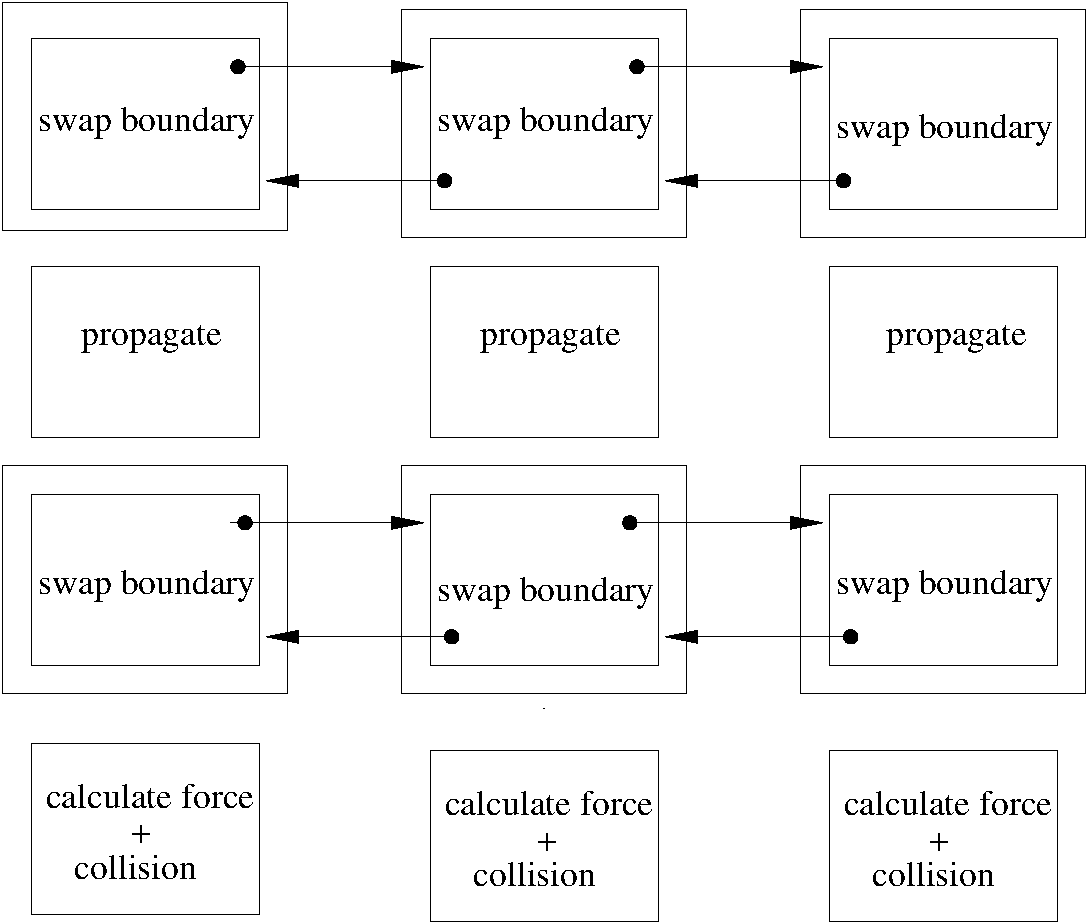
\includegraphics[width=6.20in]{parallel.pdf} &
   	\end{tabular}
   \vfill
 \caption{Flow chart of the parallel LB algorithm.}
\label{fig:flowchart}
\end{figure}

The parameters for the simulation, such as its duration, initial conditions,
and coupling parameters, are all controlled by text files, which can be
modified using any text editor.

When the code is run, it reads the input file, and performs the appropriate
simulation. If large numbers of input files are used, it may be advisable to
generate them using a simple shell or perl script.

The code prints a small amount of information to standard output, usually just
messages detailing the input parameters at the start, and a brief note when a
new time step is commenced. If desired, sanity checks can be performed after
user determined set of timesteps.

The program can be instructed to periodically write information
concerning the state of the simulation, such as the particle densities
and velocities, to disk. For reasons of efficiency, every time such
output is produced, each CPU can write a file containing information about
its own chunk of the simulation, and nothing else. These files are later tied
together to form a coherent whole, by an external postprocessor. If a small
loss of efficiency is acceptable, the code can be instructed to do the
postprocessing each time data is written to disk.

Previous versions of the code were only able to write these output files in
Fortran unformatted mode, which is platform-dependent: A postprocessor compiled
on an SGI Origin2000 will not be able to understand the output from a
simulation run on a Cray T3E.

This version of the code fully supports to additional output formats which are
both platform-independent: xdr \cite{bib:rfc1832} (using Frans van Hoesel's
XDRF library \cite{bib:Hoesel}) and ASCII. Obviously, because of its
inefficient use of disk space, ASCII output is desirable for debugging purposes
only. Today's defacto standard is parallel HDF5 output which allows the best
performance and portability if the HDF5 library is available.

If the internal postprocessing routines are not used, the external
postprocessor may be run to tie all the CPUs' outputs together to produce
output that may be visualized or used for calculation. The output from the
external postprocessor is platform-independent as it utilizes the XDR format.

\begin{figure}[!hp]
\centering
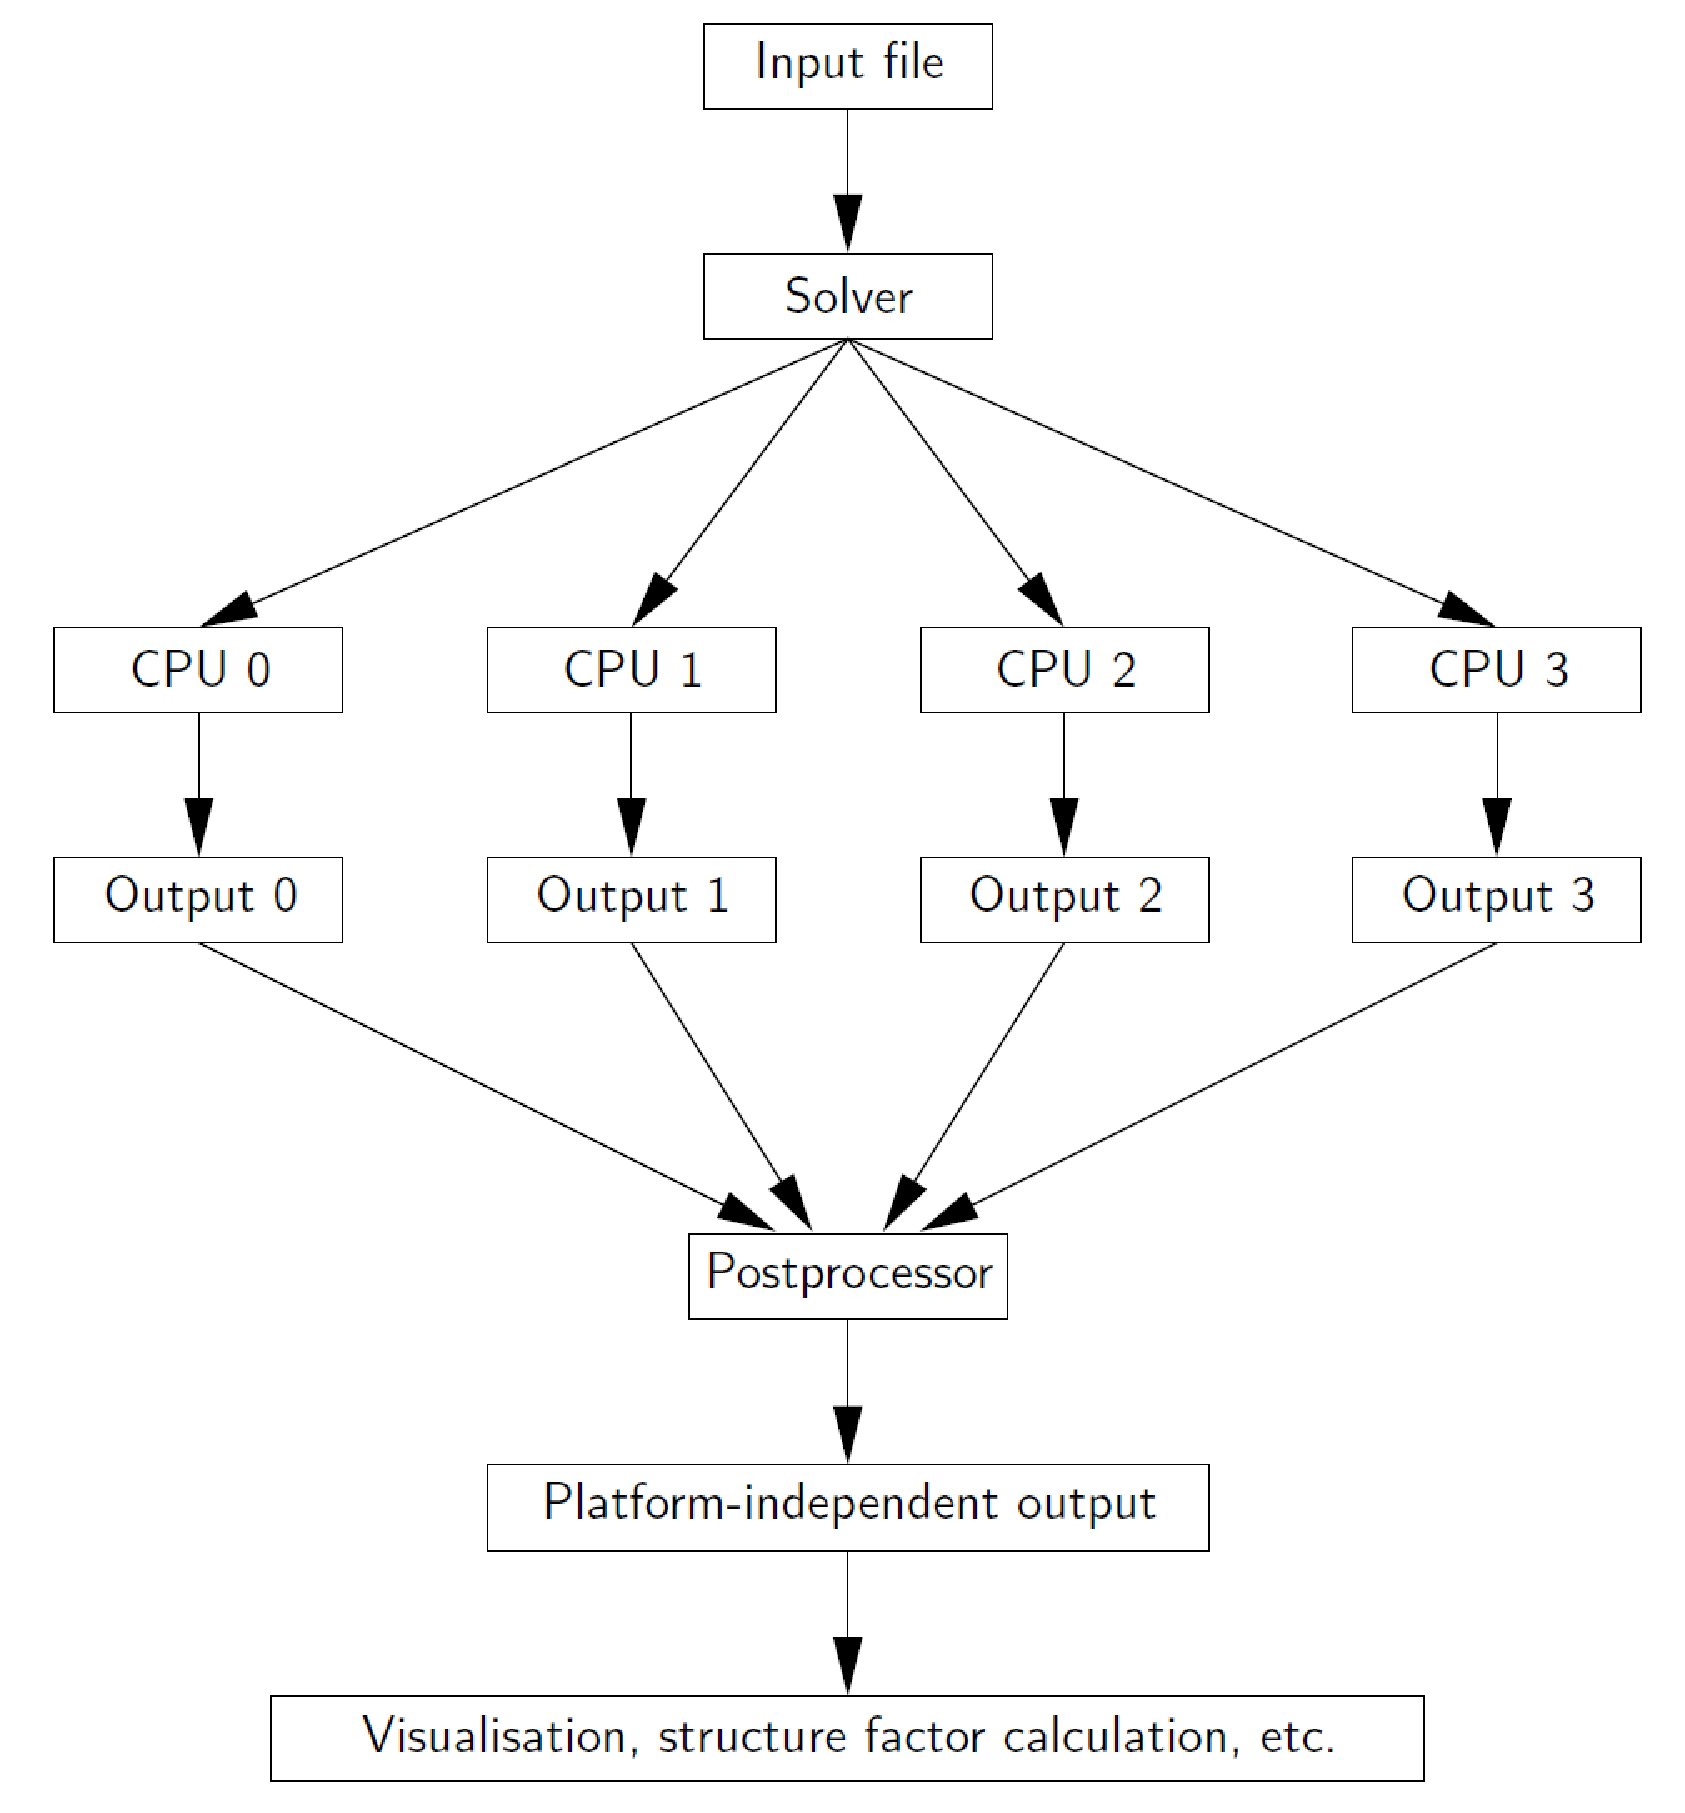
\includegraphics[width=1.0\textwidth]{lb3d_flow.pdf}
\caption{The fully parallel code.
\label{fig:parallel}
}
\end{figure}

% Try to persuade LaTeX to put the figures here..

\clearpage

\section{The LBE Algorithm}

The simulation takes place on a 3-dimensional lattice, consisting of
$n_x$ sites in the $x$-direction, $n_y$ nodes in the y-direction, and
$n_z$ sites in the $z$-direction. Each node is joined to its neighbours by
a set of lattice vectors $c_i$.
In the current implementation of the above algorithm in 3D we use 
a projected face-centred hypercubic (PFCHC) lattice \cite{bib:pfchc}.
The motivation for using this lattice is that it is known to yield 
isotropic Navier-Stokes behaviour for a single-phase fluid \cite{bib:pfchc}. 
There are in total 25 lattice vectors
joining each site to 19 neighbours - the vectors pointing in the X, Y,
and Z directions have twofold degeneracy. 

We use the notation that the vectors $c_i$ are the $i^{th}$ column 
vector of the matrix
\[
  \left(\,
  \begin{array}{ccccccccccccccccccc}
    1 & -1 & 0 &  0 & 0 &  0 & 1 &  1 & 1 &  1 & -1 & -1 & -1 & -1 & 0 &  0 &  0 &  0 & 0 \\    
    0 &  0 & 1 & -1 & 0 &  0 & 1 & -1 & 0 &  0 &  1 & -1 &  0 &  0 & 1 &  1 & -1 & -1 & 0 \\
    0 &  0 & 0 &  0 & 1 & -1 & 0 &  0 & 1 & -1 &  0 &  0 &  1 & -1 & 1 & -1 &  1 & -1 & 0 \\
  \end{array}\,
  \right)
\]
The vectors of the D3Q19 grid are illustrated in Fig.~\ref{fig_d3q19}.
\begin{figure}
\centering  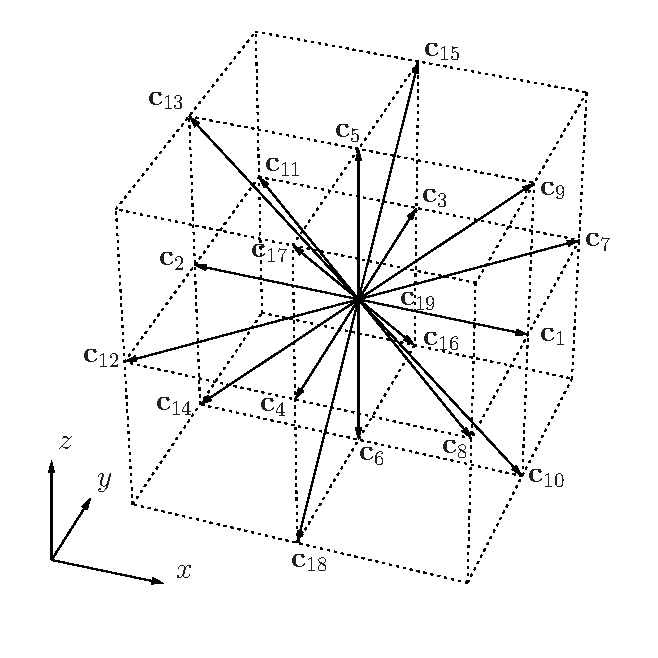
\includegraphics[width=0.6\linewidth]{d3q19.pdf}
%\includegraphics[width=\linewidth]{lbe}

\caption{The geomety of our D3Q19 lattice with the lattice vectors $\vect{c}_i$.
  \label{fig_d3q19}
}
\end{figure}

The code accounts for three fluid species: red (oil), green
(surfactant), and blue (water)- the green particles behave like dipoles,
and therefore possess orientational degrees of freedom. 
A given velocity vector at a given site will have a certain density 
$f^r_i$, $f^b_i$, $f^s_i$ of red, blue and green particles,
respectively, there will be also a net average dipole moment ${\bf
d}$, for surfactant particles at each site.
During each time step of the simulation, the following processes take
place:

\begin{itemize}
\item{\bf Advection} \\
	The particles are propagated along their velocity vectors, to
	adjacent sites. More specifically, for each site at position
	\vect{r}, the particles with velocity $\uvect{c}_i$ are moved to
	the site at position $\vect{r} + \vect{c}_i$. 

\item{\bf Collision} \\

	At each site, all the particles at that site interact: they
	collide and are redistributed. This takes place over several
	steps:

	\begin{itemize}
	\item{Calculation of Hamiltonian and dipole moments}

		A vector $\vect{h}$ is used in calculation of the
		surfactant interactions - the reader is referred to the
		papers describing the algorithm in depth for more
		detail
		\cite{bib:maziar1}
		. The new equilibrium surfactant dipole
		$\vect{d}^{eq}$ is calculated from $\vect{h}$.
	
	\item{Calculation of forces}

		At each site, the forces on each particle species are
		calculated: $\vect{F}^{cc}$, $\vect{F}^{cs}$,
		$\vect{F}^{sc}$, and $\vect{F}^{ss}$ are the forces on
		coloured particles due to other coloured particles, on
		coloured particles due to surfactants, on surfactants
		due to coloured particles, and on surfactants due to
		other surfactants, respectively.

		To use a single component multi phase (SCMP) approache, an attractive self interaction force $\vect{F}^{cc}$. To include attractive interactions the logical value
{\tt SCMP} can be set in the input-file.                

		These forces are then summed to find the net force on
		particles of a given species at that site.

	\item{Redistribution}

	At each site:

	\begin{itemize}
	\item
		The density $\rho^{\sigma}$ and fluid velocity 
                ${\bf u}^{\sigma}$ of each fluid component is computed:

	        \[
	    \rho^{\sigma}= m^{\sigma}\sum_i \; n_i^{\sigma},
                \]

	\[ 
	\rho^{\sigma} {\bf u}^\sigma = m^{\sigma}\sum_i \; {\bf c}_i n_i^{\sigma} 
	\]
	where $m^{\sigma}$ is the molecular mass of species $\sigma$.

	\item
		The average velocity $\tilde{\vect{u}}$ 
                which enters the equilibrium 
                distribution functions $n_i^{\sigma,eq}$ is calculated:
 		\[
		{\tilde {\bf u}} 
		= 
		\sum_\sigma \frac {\rho^\sigma {\bf
		u}^\sigma}{\tau_\sigma} 
		/ 
		\sum_\sigma \frac {\rho^\sigma} {\tau_\sigma}.
		\]
	\item
		The force term is calculated. 

		
	\item
		The equilibrium densities for each species for each
		velocity vector, $n^{\sigma\mathrm{(eq)}}_i$, are found.
	\item
		The collision itself takes place: the particle densities
		are adjusted through the fundamental equation of the LBE
		model:

		\[
			n^{\sigma}_i \leftarrow
					n^{\sigma}_i -
					\frac 1 {\tau^{\sigma}}
					\left(
						n^{\sigma}_i -
						n^{\sigma\mathrm{(eq)}}_i
					\right)
		\]

		

	\end{itemize}
	\end{itemize}

\end{itemize}


\section{Installing LB3D}

\subsection{Platforms and portability}

The code should compile and run on any 64-bit UNIX (Such as Compaq Tru64, SGI
Irix, IBM AIX, or Linux running on Ultrasparc, Alpha or SGI ALTIX, etc.) with
very little, if any, modification.

Porting the code to a 32-bit platform is possible, however, it should be noted
that there will be some loss of accuracy and the size of the simulated system
will be limited due to the 2GB memory limit.

\subsection{Requirements}

The following are required to install LB3D:

\begin{itemize}
\item A 64-bit UNIX platform as detailed above.
\item A Fortran 90 compiler that supports memory autodeallocation (the only compiler we know and that does not support this feature are at least the early versions of the Portland Group compiler.)
\item An ANSI C compiler
\item The MPI libraries
\item Perl version 5 is required for the postprocessor.
\item For platform-independent output, the system should support the Sun
	Microsystems RPC interface. The authors are not aware of any
	existing UNIX platforms which fail to meet this criterion, since
	it is required for the Sun Network Filing System (NFS).
\item The GNU {\tt gmake} utility
\item The UNIX {\tt tar} utility
\item The UNIX {\tt patch} utility
\item The XDRF library (included in this distribution)
\item Parallel HDF5 if the postprocessing is supposed to be done with HDF5. (Obtainable from {\tt http://www.hdfgroup.org}) 
\end{itemize}

Furthermore to rebuild the documentation files from sources are required:

\begin{itemize}
\item Doxygen
\item A LaTeX distribution including {\tt pdflatex}
\end{itemize}

The testing script {\tt testLB3D.sh} currently relies on both XDR- and HDF5-support present.

\subsection{Setup LB3D}

\subsubsection{Unpacking}

Stable versions of the code are distributed as gzipped tar files: for
example, {\tt lb3d-2012-03-09.tgz}. Copy this file into the
directory into which you wish to install the program then type:
\begin{verbatim}
% tar xvzf lb3d-2012-03-12.tgz
\end{verbatim}
This will uncompress and unpack the distribution. All files will be
unpacked into a directory called {\tt lb3d}.\\

\subsubsection{Compiling the parallel HDF5 library}

\vspace{2em}
\colorbox{lightgray}{\parbox{\textwidth}
{
  \vskip10pt
  \leftskip10pt
  \rightskip10pt


{Please Note: For large scale production runs the use of parallel HDF5 output is strongly recommended. The use of the library is however optional. If you like to omit this step, be sure to set {\tt dump\_format = 'xdr'} in the {\tt \&lbe\_input}-section of the input file.
}
}}
\vspace{2em}

First of all, you need a parallel compiler and environment, i.e. a working
MPI implementation. If this is not the case, first of all get one, e.g.,
MPICH2, from

\verb|http://www.mcs.anl.gov/research/projects/mpich2/|

configure it. You have to enable the fortran bindings and the parallel IO:

\begin{verbatim}
configure  --enable-f77 --enable-f90 --enable-romio  \
  --build=x86_64 --prefix=/path/to/your/mpidir
\end{verbatim}

Note that not every version works on all platforms with all compilers. I got
the version 1.0.7 compiled with intel and the version 1.0.8 with gcc under 
OpenSuse 11.

I recommend to install it somewhere, e.g., in \verb|$HOME/local/stow/mpich2-intel/|,
and then install it with the tool \verb|stow| to the actual place.

To build it with the intel compilers, you first have to set the correct 
environment variables so that the intel compiler works correctly. There are 
different versions for different platforms, the version with ``cce'' and ``fce''
are for 64-bit, the ones without ``e'' are for 32 bit, e.g. itanium.
\begin{verbatim}
 export F77=/usr/local64/intel/fce/9.1.040/bin/ifort
 export F90=/usr/local64/intel/fce/9.1.040/bin/ifort
 export FFLAGS="-I/usr/local64/intel/fce/9.1.045/include/ -I/usr/local/include/ \
   -I/usr/include/ -I/usr/include/sys/ -I/usr/include/linux"
 export CFLAGS="-I/usr/local64/intel/cce/9.1.045/include/ -I/usr/local/include/ \
   -I/usr/include/ -I/usr/include/sys/ -I/usr/include/linux"
 export LDFLAGS="-L/usr/local64/intel/cce/9.1.040/lib/ -L/usr/lib64/"
 export CC=/usr/local64/intel/cce/9.1.045/bin/icc
\end{verbatim}

now configure, compile (make) and install (make install; cd somewhere; stow ). 
Then, you have parallel compilers.
With these you can compile HDF5. First, you have to compile the compression 
filters. With this you have to 

\begin{verbatim}
 export F77=/path/to/your/mpif77
 export F90=/path/to/your/mpif90
 export F9X=/path/to/your/mpif90
 export CC=/path/to/your/mpicc
 export FFLAGS="-I/your/local/include/dir"
 export CFLAGS="-I/your/local/include/dir"
 export LDFLAGS="-L/your/local/lib/dir"
\end{verbatim}

Now, configure, make, make install, and stow the libraries szlib and/or zlib.
(They are mentioned on the HDF5 homepage as ``External Software''),
Finally, get the HDF sources from \verb|http://www.hdfgroup.org/HDF5/|.

The main problem in compiling HDF might be, that some HDF headers are installed 
on your system, but these headers might belong to a different version of HDF.
With the intel compilers I managed to work around by means of the CFLAGS:

\begin{verbatim}
 export CFLAGS="-iquote. -iquote/sourcedir/hdf5-1.8.2/src/ \ 
   -I/sourcedir/hdf5-1.8.2/src/"
\end{verbatim}

For gnu compilers ``\verb+-I+'' might work, too, but with intel this switch has 
a different meaning. One problem, including the source
directory with the ``\verb+-iquote+'' directive is, that you may not delete the sources
after you have installed everything. A possible way out of this, is to compile HDF a 
second time, with the already installed headers in the CFLAGS and install the 
version obtained this way over the firstly installed one. If you do so, you might 
have to copy all headers from the src directory to the include directory at the 
place you install the hdf5.

\begin{verbatim}
configure  --enable-parallel --enable-fortran --disable-cxx --disable-hl \
 --build=x86_64 --prefix=/your/install/dir --filters=zlib
\end{verbatim}

This is the first step without the ``high level functions''. So, after the 
first install, you should reconfigure and omit the flag ``\verb+--disable-hl+''. 
If another installation of hdf5 -- maybe in a different version
exists on your system, you should take care that the correct headers are included.
I had to go to the source directory hl/src and edit the header files there. Every
occurence of \verb+#include <hdf5.h>+ has to be replaced by \verb+#include "hdf5.h"+.
Perhaps there is a way around this modification by means of the \verb+-iquote+ switch
in the CFLAGS. Note that \verb/C++/-bindings cannot be compiled together with 
parallel IO. Therefore, the \verb/C++/-bindings have to be disabled.

For linking lb3d to the hdf library, the fortran module files are needed. However, 
these are generated in the src directory, but they are not installed by default.
It makes sense to copy them manually to the lib directory, where your \verb+libhdf5.a+
is installed.

The compression filters can be internal or external. If you specify them with 
``\verb+--filters=+\dots'', they are compiled into the hdf-library, otherwise you 
have to add ``-lz'' to the line ``\verb+LIBSHDF =+ \dots'' 
in \verb+Makefile.template+  when 
compiling lb3d. -- By the way: You have to adjust the paths in the  \verb+Makefile.template+ anyway -- or, even better: create a new \verb+.defines+-file
for your platform.

Note that \verb|h5utils| is another package. Since this is used for postprocessing,
it may be useful to recompile HDF5 in a serial version and link h5utils against 
that one. Since it might not be possible to link it statically, it is perhaps a
good idea, to copy the serial hdf5-library into the install directory of h5utils
to some non-standard path and add that path to the \verb+$LD_LIBRARY_PATH+ variable in
the .bashrc. (This section was written by Martin Hecht)

\subsubsection{Configuring and compiling}
\label{sec:configCompile}

Before compiling, a script needs to be run which sets certain options
which vary across platforms. To do this, in the directory lb3d execute:
\begin{verbatim}
% ./configLB3D.sh CONFIG PLATFORM COMPILER_OPTIONS
\end{verbatim}
where PLATFORM is one of LINUX64, HECTOR, HUYGENS, JUGENE, JUROPA.

\vspace{2em}
\colorbox
{lightgray}{\parbox{\textwidth}
{
  \vskip10pt
  \leftskip10pt
  \rightskip10pt


{Please Note: LB3D is as of yet not using autoconf. Therefore it is likely that you have to adjust the {\tt defines.PLATFORM} file for the compilation to be successful  \vskip10pt}
}
}\vspace{2em}

Compiler options are passed through to all Makefiles. The script {\tt find\_flags.sh}, when run in the code directory, will give a report on all the flags currently being used in precompiler directives.~\\

To build a the code for simulation of a ternary system with XDR and HDF-output supported issue:
\begin{verbatim}
% ./configLB3D.sh CONFIG PLATFORM -DUSEXDRF -DUSEHDF 
\end{verbatim}
For binary systems define {\tt NOSURFACTANT}
\begin{verbatim}
% ./configLB3D.sh CONFIG PLATFORM -DUSEXDRF -DUSEHDF -DNOSURFACTANT
\end{verbatim}
For a single fluid component define {\tt SINGLEFLUID}
\begin{verbatim}
% ./configLB3D.sh CONFIG PLATFORM -DUSEXDRF -DUSEHDF -DSINGLEFLUID 
\end{verbatim}

See appendix \ref{apx:compileOptions} for a list of the current state with short descriptions.

And then type~\\
\begin{verbatim}
% ./configLB3D.sh MAKE
\end{verbatim}
to compile the code.

\subsubsection{Tests}

LB3D comes with a simple testing facility in form of a runscript hat executes various small simulations involving different functionalities and compares the results to reference results. Currently tested are:
\begin{itemize}
\item the Lees-Edwards boundary condition for a binary mixture 
\item The body force (``gravitation'') for a ternary mixture
\item Zou-He velocity boundary condition for a ternary mixture
\item The parameter set for the formation of a gyroid in a ternary mixture
\item The wettability-model of our bounce back boundary for a binary mixture
\end{itemize}

Before running the Tests, please review the file /lb3d/testLB3D.sh, where you find further details and most likely will like to adjust basic settings. To execute the tests then execute the script:

\begin{verbatim}
% ./testLB3D.sh
\end{verbatim}
\vspace{2em}
\colorbox
{lightgray}{\parbox{\textwidth}
{
  \vskip10pt
  \leftskip10pt
  \rightskip10pt


{Please Note: This feature was introduced recently and has not been extensively tested across platforms itself. If you have not altered the code and a binary was created, a failing test may point rather to an issue of the testing facility. If you run into problems, please let us know by an email to \maintainer.}
}
}\vspace{2em}


\subsubsection{Possible problems}

The problems described below may occur when the code is compiled or run
on platforms on which it has not been tested. In these cases, an email
to the maintainer (currently \maintainer), describing any problems and
possible cures or workarounds, would be useful, since the fixes may then
be incorporated into the next version of the code.

\begin{description}

{\item [ The program fails on startup. ]
\ \\

If you see the error message:

\begin{verbatim}
lib-1304 ./lb3d: UNRECOVERABLE library error 
  Namelist input group name "FIXED_INPUT" does not
  match READ group name.
\end{verbatim}

Then edit the {\tt Makefile} so that at least one line at the start
reads:

\begin{verbatim}
IO_INIT= -DIO_INIT
\end{verbatim}

This corrects a quirk in the way some Fortran libraries treat namelist
input. Email the maintainer, since this should be detected in the {\tt
configure} script.

Alternatively, the error message:

\begin{verbatim}
sys-2 : UNRECOVERABLE error on system request 
  No such file or directory

Encountered during an OPEN of unit 10
Fortran unit 10 is not connected
IOT Trap
\end{verbatim}

may mean that the directory specified by {\tt folder} does not exist in the
output directory.

}
{\item [ The compile fails. ]
\ \\

        Make sure that all required libraries are present and that the the settings in {\tt defines.PLATFORM} match your systems configuration.

        Email the maintainer (\maintainer).
}

\end{description}





\newpage
\section{Running LB3D}

\subsection{Invoking LB3D}

For debugging and testing, the code may be run interactively using the
{\tt mpirun} command. 

\begin{verbatim}
% cd /path/to/executable/lb3d
% mpirun -np <#cpu> ./lb3d -f <input-file> [-d <diff-input>] [-r <restore-string>]
\end{verbatim}

This will run the solver with \#cpus CPUs; vary the argument following
{\tt -np} to vary the number of CPUs used. Be aware that only certain
numbers of CPUs will be possible, depending on the shape and size of the
lattice. Explicitely setting the MPI domain decomposition in the {\tt fixed\_input}-section of the input-file may help to make exotic domain sizes work (See section \ref{sec:fixedInput}).

The parameters controlling the LB3D simulation are all contained in one
file, the input file. The path to the input file is set via the commandline-argument {\tt -f {\textless}input-file{\textgreater}}. See section \ref{sec:inputFile} for details on the file format and the available settings.



\subsubsection{Commandline parameters}

\begin{description}
\item [-f {\textless}input-file{\textgreater}] mandatory~\\Specify the input-file
\item [-d {\textless}diff-input{\textgreater}] optional~\\Specify a differential input-file. The differential input-file may contain a subset of the input-file parameters that will override the settings in the input-file provided via {\tt -f}. This is intended to ease the creation of input for parameter sweeps and helps keeping an overview of the parameters relevant to a particular simulation.
\item [-r {\textless}restore-string{\textgreater}] optional~\\
Specify a restore-string in the form {\tt t00000000-0000000000}, where the first eight digits specify a timestep and the latter ten digits a simulation ID. If a suiting checkpoint is found in the path provided as {\tt srccpfolder} in the {\tt \&variable\_input} section of the input file (default is the directory of the binary {\tt '.'}), the simulation data will be restored from checkpoint. 

\end{description}

\subsubsection{Submitting to a batch queue }

For serious jobs, it is likely that the code will be launched from a
batch queue system. It is highly recommended that the documentation for
the specific system used is read carefully, since batch queue systems
may vary widely in their behaviour.

The following script illustrates how to submit a $64$ processor lb3d job to a machine with 32 cores per node using the Portable Batch System (PBS).

\begin{verbatim}
# A PBS Example
# Note that #PBS at the start of a line designates PBS instructions
# rather than mere comments.

# Give the job a name
#PBS -N jobname

# Specify files to write standard out and standard error streams to
#PBS -e jobname.err
#PBS -o jobname.log

# Specify an e-mail address
#PBS -M username@mailhost

# Send e-mail notification on job (a)bort (b)egin (e)nd 
#PBS -m abe

# Request 2 nodes with 32 processes per node
#PBS -l nodes=2:ppn=32

# Request 512 megabyte of RAM
#PBS -l mem=512mb

# Request a the resources for 2 hours
#PBS -l walltime=02:00:00

# The remainder is treated as a shell script executed at job start
# The following variables are available on job execution
# 
# Nodename $PBS_NODEFILE
# Hostname $PBS_O_HOST
# Originating queue $PBS_O_QUEUE
# Actual queue $PBS_QUEUE
# Working directory $PBS_O_WORKDIR
# Environment vars $PBS_ENVIRONMENT
# Job ID $PBS_JOBID
# Jobname $PBS_JOBNAME
# Home directory $PBS_O_HOME
# Path variable $PBS_O_PATH

echo Simulation start $(date)

cd $PBS_O_WORKDIR
mpirun -n 64 ./lb3d -f input-file

echo Simulation End $(date)
# EOF PBS Example
\end{verbatim}

In interactive mode (where available), the binary can be invoked using an entry in the shell script like:
\begin{verbatim}
% mpirun -np 64 ./lb3d -f <input-file>
\end{verbatim}

To submit the job to the batch system type 
\begin{verbatim}
% qsub scriptname 
\end{verbatim}

Here ``scriptname'' is the name of the file which contains the above script.


\subsection{The input-file}
\label{sec:inputFile}

The input file is an ASCII file, in Fortran ``namelist'' format.
Essentially, it consists of three sections named {\tt fixed\_input}, {\tt
variable\_input}, and {\tt lbe\_input}. 

Each section consists of a set of key-value pairs, corresponding to
simulation parameters. It is recommended that these pairs are separated
by a newline.

Note that string values should be delimited by single quotes (``{\tt '}''). An example can be found in appendix~\ref{apx:inputFile}.

\subsubsection{The {\tt fixed\_input} section}
\label{sec:fixedInput}
The dimensions of the lattice are specified by {\tt nx}, {\tt ny}, and
{\tt nz}. The random number seed, {\tt seed} is used only in generating
random initial conditions.

\begin{center}
\begin{tabular}{|l|l|p{0.5\textwidth}|}
\hline
Variable name	&	Default value	&	Meaning \\
\hline
{\tt nx }	&	{\tt 16 }	&	
		The size of the lattice in the X direction.\\
\hline
{\tt ny }	&	{\tt 16 }	&
		The size of the lattice in the Y direction.\\
\hline
{\tt nz }	&	{\tt 16 }	&
		The size of the lattice in the Z direction.\\
\hline
{\tt seed }	&	{\tt 1 }	&
		The random number seed. This is used in setting up
		randomized initial conditions.\\
\hline
{\tt obs\_file }	&	{\tt 'empty.dat' }	&
		This is the name of the file containing the rock
		geometry data to be loaded. If it is set to 
		{\tt 'empty.dat'}, no rock file will be loaded.\\
\hline
{\tt boundary\_cond }	&	{\tt 0 }	&
		set to nonzero value for invasive or sheared flow.\\
\hline
{\tt cdx } & {\tt 0 }  &
    The size of the MPI Cartesian grid in the x-direction.
    If set to zero or if not defined, MPI will decide. \\
\hline
{\tt cdy } & {\tt 0 }  &
    The size of the MPI Cartesian grid in the y-direction.
    If set to zero or if not defined, MPI will decide. \\
\hline
{\tt cdz } & {\tt 0 }  &
    The size of the MPI Cartesian grid in the z-direction.
    If set to zero or if not defined, MPI will decide. \\
\hline



\end{tabular}
\end{center}

\newpage

\subsubsection{The {\tt variable\_input} section}

The parameters in this section control aspects such as which output
files to write, how often to write them, and what to call them, as
well as how long to run the simulation for. Do not set the n\_sci\_
parameters to 0, even if the matching sci\_ parameter is set to .false.!

\begin{center}
\begin{longtable}{|l|l|p{0.5\textwidth}|}
\hline
Variable name	&	Default value	& Meaning	\\
\hline 
{\tt n\_iteration  }	&	{\tt 10 }	&
		The number of time steps for which the simulation will
		run.\\
{\tt n\_sci\_start  }	&	{\tt 0 }	&
		Start of science output at this time step. \\
{\tt sci\_int  }	&	{\tt \ffalse }	&
		Write the colour field? \\
{\tt n\_sci\_int  }  & {\tt 100 }  & 
    The colour output will be written every {\tt n\_sci}
    time steps.\\
{\tt sci\_sur  }	&	{\tt \ffalse }	&
		Write the surfactant density? \\
{\tt n\_sci\_sur  }	&	{\tt 100 }	&
		The surfactant density will be written every {\tt n\_sci\_sur}
		time steps.\\
{\tt sci\_od  }	&	{\tt \ffalse }	&
		Write the oil densities? \\
{\tt n\_sci\_od  }	&	{\tt 100 }	&
		The oil densities will be written every 
		{\tt n\_sci\_od} time steps.\\
{\tt sci\_wd  }	&	{\tt \ffalse }	&
		Write the water densities? \\
{\tt n\_sci\_wd  }	&	{\tt 100 }	&
		The water densities will be written every 
		{\tt n\_sci\_wd} time steps.\\
{\tt sci\_dir  }	&	{\tt \ffalse }	&
		Write the surfactant directions? \\
{\tt n\_sci\_dir  }	&	{\tt 100 }	&
		The surfactant directions will be written every
		{\tt n\_sci\_dir}  time steps.\\		
{\tt sci\_vel  }	&	{\tt \ffalse }	&
		Write the mixture's Z-velocity as an average over all
		the species, according to Eq.~\eqref{Z-VELOCITY}) of
		Subsec.~\ref{OUTPUT-FILES}. \\
{\tt n\_sci\_vel  }	&	{\tt 100 }	&
		The mixture's Z-velocity as an average over all the
		species will be written every {\tt n\_sci\_vel}  time
		steps.\\		 
{\tt sci\_flo  }	&	{\tt \ffalse }	&
		Write the total Z-velocities for each component. \\
{\tt n\_sci\_flo  }	&	{\tt 100 }	&
		The total Z-velocities for each component will be written every
		{\tt n\_sci\_flo}  time steps.\\		
{\tt sci\_arrows  }	&	{\tt \ffalse }	&
		Write the total linear momentum density. \\
{\tt n\_sci\_arrows  }	&	{\tt 100 }	&
		The total linear momentum density will be written every
		{\tt n\_sci\_arrows}  time steps.\\		
{\tt sci\_rock  }	&	{\tt \ffalse }	& Write the rock\_state at each lattice node. \\
{\tt n\_sci\_rock  }	&	{\tt 100 }	& The rock\_state at each lattice node will be written every {\tt n\_sci\_rock} time steps.\\
{\tt sci\_pressure}	&	{\tt \ffalse }  & Write pressure? \\
{\tt n\_sci\_pressure}     & {\tt 100 }        & Write the pressure every {\tt n\_sci\_pressure} time steps.\\
{\tt sci\_pressure\_init} & {\tt 100 }        &
    Initial condition for pressure calculation. Should differ from init\_cond only if we are restoring.\\
{\tt post }	&	{\tt \ffalse }	&
		Use internal postprocessing.\\
{\tt folder  }	&	{\tt 'binary' }	& Output file folder (should be
created by user prior to execution of the code). \\
{\tt gr\_out\_file  }	&	{\tt 'test' }	& Output file prefix. \\
{\tt init\_cond  }	&	{\tt 0 }	& Determines the initial conditions of the simulation.\\
{\tt restore}           &       {\tt .false. }  & When set to true, simulation will be restored from checkpoint. This has the same effect as setting init\_cond = 7. \\
{\tt inv\_fluid  }	&	{\tt 0 }	& Specifies the type of invading fluid.\\
{\tt inv\_type  }	&	{\tt 0 }	& Several invasion types use {\tt inv\_type} to specify a sub-type.\\
{\tt fr  }	&	{\tt 1.0 }	& Parameter related to the density of the
red (oil) particles used for many initial conditions and invasion implementation. \\
{\tt fb  }	&	{\tt 0.5 }	& Parameter related to the density of the
blue (water) particles used for many initial conditions and invasion implementation. \\
{\tt fg  }	&	{\tt 0.1 }	& Parameter related to the density of surfactant
 used by many initial conditions and invasion implementation. \\
{\tt fd  }	&	{\tt 0 }	& Parameter related to the dipole orientation.\\
{\tt fr1  }	&	{\tt 0.2 }	& Size parameter for lamellae or bubbles. \\
{\tt fr2  }	&	{\tt 0.3 }	& Another size parameter.\\
{\tt pr  }	&	{\tt 0.5 }	& Another parameter related to the density of the
red (oil) particles used for many initial conditions and invasion implementation. \\
{\tt pb  }	&	{\tt 1.0 }	& Another parameter related to the density of the
blue (water) particles used for many initial conditions and invasion implementation. \\
{\tt pg  }	&	{\tt 0.1 }	& Another parameter related to the density of surfactant
 used by many initial conditions and invasion implementation. \\
{\tt fd  }	&	{\tt 0 }	& Another parameter related to the dipole orientation.\\
{\tt qr  }	&	{\tt 0.5 }	& Another parameter related to the density of the
red (oil) particles used for many initial conditions and invasion implementation. \\
{\tt qb  }	&	{\tt 0.5 }	& Another parameter related to the density of the
blue (water) particles used for many initial conditions and invasion implementation. \\
{\tt qg  }	&	{\tt 0.1 }	& Another parameter related to the density of surfactant
 used by many initial conditions and invasion implementation. \\
{\tt qd  }	&	{\tt 0 }	& Another parameter related to the dipole orientation.\\
{\tt rock\_colour  }	&	{\tt 0 }	&
		Specifies the colour of the rock sites. \\
{\tt beta  }	&	{\tt 1.000000 }	& Inverse temperature for dipole orientation.\\
% \hline
% \end{tabular}
% \end{center}
% \begin{center}
% \begin{tabular}{|l|l|p{90mm}|}
% \hline
% Variable name	&	Default value	& Meaning	\\
% \hline
{\tt drop\_Xshift } &      {\tt 0}         &
                With {\tt init\_cond=14}: Shift the droplet in direction X=\{x,y,z\}.\\

\hline
\end{longtable}
\end{center}

\subsubsection{The {\tt lbe\_input} section}

These parameters control aspects specific to the Lattice-Boltzmann method,
such as relaxation times. For example, the kinematic viscosity $\nu^{\sigma}$
of of each fluid component $\sigma$ is related to the relaxation time
parameter $\tau^{\sigma}$ through the relation \cite{bib:maziar1} $\nu^\sigma
= (\tau^{\sigma}- 1/2)/\beta_0$, with $\beta_0=3$ for the 19 velocity vector
model implemented in the present version of the code. In case of binary
applications these parameters also control the immiscibility of the
system. For example, in a binary system with equal densities of oil and water,
equal relaxation times $\tau_b=\tau_r=\tau$ and equal masses {\tt
  amass\_b=amass\_r=m}, the theoretical critical value of water-oil coupling
$g_{br}^c$ beyond which the system phase separates is given by
\cite{bib:shan-chen} $ g_{br}^{c}= m(\tau-1/2)/(\tau b \bar{n})$, where $b$ is
the number of non-zero velocity vectors and $\bar{n}$ is the average density
of the fluid.

\bigskip


\bigskip

The {\tt bdist} parameter specifies the form of the equilibrium distribution
function. 

\bigskip

\begin{tabular}{|l|p{115mm}|}
	\hline
{\tt bdist} value	&	Meaning	\\
	\hline
{\tt 0  }	& Equilibrium distribution function described in
		\cite{bib:maziar2}, with additional cubic terms. \\
{\tt 1  }	& `Chen operator' based on an exponential form of the
equilibrium distribution this ensures densities are always positive. However,
neither momentum nor particle number are exactly conserved.\\
{\tt 2 }	& Equilibrium distribution as described in \cite{bib:maziar1}.
The non-linear force terms provide extra stability, but are not consistent with
discretization of the Boltzmann equation in the presence of forces.\\
{\tt 3 }	& Equilibrium distribution function described in
		\cite{bib:maziar2}.\\
{\tt 4 }	& A second order version of of the equilibrium distribution
function ({\tt 2}). Force implementation by~\cite{PhysRevE.65.046308}. \\
{\tt 5 }	& A third order version of the equilibrium distribution function. Force implementation
following~\cite{PhysRevE.65.046308}. \\

\hline
\end{tabular}

\bigskip

The Shan-Chen forces depend on an effective number density, given by
$\psi^\sigma (n^\sigma )$ \cite{bib:shan-chen}; the {\tt psifunc} parameter lets
you choose its functional form. To make use of this feature, the program has to be compiled with the option {\tt COMPAT\_PSIFUN} (See section \ref{sec:configCompile}, appendix \ref{apx:compileOptions}).

\bigskip

\begin{tabular}{|l|l|}
	\hline
{\tt psifunc} value	&	Meaning	\\
	\hline
{\tt 0  }	& Original code $\psi^\sigma = n^\sigma$, but with clipping of
the force for high $n^\sigma$.\\
{\tt 1  }	& $\psi^\sigma = n^\sigma$, no clipping.\\
{\tt 2 }	& $\psi^\sigma = 1 - e^{-n^\sigma}$, no clipping.\\
	\hline
\end{tabular}

\begin{center}
\begin{tabular}{|l|l|p{88mm}|}
\hline
Variable name	&	Default value	& Meaning	\\
\hline
{\tt SCMP } &{\tt \ftrue} & Enable single component Shan-Chen interactions.\\
{\tt ZEROFORCEOFFSET } &{\tt \ftrue} & Non-interacting wall. A fluid density
on the wall is set equal to the neighbor fluid average. \\
{\tt ZFOSdiag } &{\tt \ffalse} & ZEROFORCEOFFSET option. Average calculated not using the diagonal
direction. \\
\hline
\end{tabular}
\end{center}



\newpage

\subsection{Initial conditions}
The shape and size of the lattice are specified by the variables {\tt
nx}, {\tt ny}, and {\tt nz}. Before the simulation begins, the lattice
sites are populated according to the initial conditions specified in the
input file. The most important variable controlling these is 
{\tt init\_cond}. At present, it may take one of 17 values:

\begin{description}
\item[-5: Constant $z$-velocity]\ \\
  puts the equilibrium distributions for $z$-velocities {\tt pr}, {\tt pb},
  and {\tt pg} for the respective fluid species on the lattice sites. The
  densities are set to the values {\tt fr}, {\tt fb}, and {\tt fg} for the
  respective fluid species. The parameter {\tt fd} defines the dipole, when
  {\tt fd}=0 $d$ is randomly distributed, otherwise the dipole is set to the
  value (0,1,0). This initial condition is available for the compilation
  option NOSURFACTANT and also SINGLEFLUID.

\item[-4: Constant density]\ \\
  puts the equilibrium distributions on the lattice sites. The densities are
  set to the values {\tt fr}, {\tt fb}, and {\tt fg}. The parameter {\tt fd}
  defines the dipole, when {\tt fd}=0 $d$ is randomly distributed, otherwise
  the dipole is set to the value (0,1,0). In the case of SINGLEFLUID and {\tt
    inv\_type}=11 the density is set by a linear interpolation of the values
  {\tt fr} at $z=1$ and {\tt pr} at $z=n_{z}$. This initial condition is
  available for the compilation option NOSURFACTANT and also SINGLEFLUID.

\item[-3: Ratio]\ \\
  gives each site the density through the equilibrium distributions specified
  in {\tt fr}, {\tt fb} and {\tt fg} for the respective fluid species. $d$ is
  set randomly. This initial condition is in fact redundant with using {\tt
    init\_cond}=-4 and {\tt fd}$\neq 1$, and for this reason can be remove in
  future version.

\item[-1: Random]\ \\
  Each species, on each lattice vector, on each site is given a density chosen
  randomly in the range [0,{\tt fr}], [0,{\tt fb}], and [0,{\tt fg}] for the
  fluid species. Used for debugging and compatibility with ME3D only. The
  dipole is set also randomly. 

\item[0: Fractional random]\ \\
  For a given species, each vector on each site is assigned an occupation
  number between zero and the fraction specified in the input-file. For
  example, if {\tt fr} is set to $1.0$, each site will have a red density
  between $0.0$ and $1.0$, and the average density of red particles will be
  $0.5$. The input parameters {\tt fb} and {\tt fg} define the density of blue
  component and surfactant. The dipole randomly distributed.

\item[1: Lamellae in the $x$-direction plus surfactant]\ \\
  This produces successive lamellae, in planes perpendicular to the
  $x$-axis. Specifically, it creates a plane of width {\tt fr1} sites with
  densities {\tt fr}, {\tt fb}, and {\tt fg} for the fluid species, followed
  by a one-site-wide layer with densities {\tt qr}, {\tt qb}, and {\tt qg} ,
  followed by {\tt fr2} sites with densities {\tt pr}, {\tt pb}, and {\tt pg}
  for the fluid species followed by another surfactant monolayer. The
  parameter {\tt fd}, {\tt qd}, and {\tt pd} define the dipole and the three
  layer, when the parameter is 0 $d$ is randomly distributed, otherwise the
  dipole is set to the value (0,1,0). It also available this initial condition for
  the compilation option NOSURFACTANT and also SINGLEFLUID. All the densities
  are set by the equilibrium distribution function.

\item[2: Lamellae in the $y$-direction plus surfactant]\ \\
  This is identical to the $x$-lamellae plus surfactant option, except that
  the layers run perpendicular to the $y$-axis. 

\item[3: Lamellae in the $z$-direction plus surfactant]\ \\
  This is identical to the $x$-lamellae plus surfactant and $y$-lamellae
  option, except that the layers run perpendicular to the $z$-axis.

% \item[4: Droplet]\ \\
%   This option produces a spherical droplet, containing a layer of oil,
%   surrounded by surfactant, surrounded by water. The size of the layers is
%   specified as a fraction {\tt fr1} or {\tt fr2} of the total system size.
%   The oil region is at the centre, and runs to a radius of {\tt fr1}: each
%   vector at site in this region is assigned an oil density of {\tt fr}.  The
%   surfactant, of density {\tt fg}, surrounds the oil, and runs from a radius
%   of {\tt fr1} to {\tt fr2}; the surfactant dipoles all point outwards,
%   towards the water.  Finally, any remaining space is filled by water of
%   density {\tt fb}.

% \item[5: Surfactant vesicle]\ \\
%   This produces a two-phase system containing water of density {\tt fb} out to
%   a radius of {\tt fr1}, surrounded by a shell containing surfactant of
%   density {\tt fg}, out to a radius {\tt fr2}. The outer sites contain water
%   at density {\tt fb}.

% \item[6: Oil vesicle]\ \\
%   This produces a two-phase system containing water of density
%   {\tt fb} out to a radius of {\tt fr1}, surrounded by a
%   shell containing oil of density {\tt fr}, out to a
%   radius {\tt fr2}. The outer sites contain water at density
%   {\tt fb}.


\item[7: Restore state]\ \\
   Initializes the lattice using checkpoint files from a previous run. The
   simulation starts from a checkpoint specified by the {\tt restore\_string}
   variable.  Checkpoint files are outputted every {\tt checkpoint} time
   steps. The input-file may change between runs, but all simulation
   parameters are supposed to be overwritten with their checkpointed
   state. However, {\tt nx}, {\tt ny} and {\tt nz} and the number of
   processors the simulation is run on must remain the same.

\item[9: Upscaler]\ \\
  Scales up a previously saved checkpoint to the new system size by
  cloning. Needs file {\tt upscale.dat}.

\item[10: Cutout]\ \\
   Cuts out a chunk from a checkpoint and puts it at an arbitrary place in the
   new system. Needs file cutout.dat. The remaining system is filled using
   initial condition -3.

 \item[11: Bi-Lamellae in the $x$-direction]\ \\
   This produces 2 successive lamellae, in planes perpendicular to the
   $x$-axis.  Specifically, it creates a plane of width {\tt fr1} sites with
   densities {\tt fr}, {\tt fb}, and {\tt fg} for the fluid species, followed
   by {\tt fr2} sites with densities {\tt pr}, {\tt pb}, {\tt pg} for the
   fluid species. The parameter {\tt fd} and {\tt pd} define the dipole and
   the two layer, when the parameter is 0 $d$ is randomly distributed,
   otherwise the dipole is set to the value (0,1,0). It also available this
   initial condition for the compilation option NOSURFACTANT and also
   SINGLEFLUID. All the densities are set by the equilibrium distribution
   function.

\item[12: Bi-Lamellae in the $y$-direction]\ \\
  This is identical to the bi-$x$-lamellae option, except that the layers run
  perpendicular to the $y$-axis.

\item[13: Bi-Lamellae in the $z$-direction]\ \\
  This is identical to the bi-$x$-lamellae and bi-$y$-lamellae option, except
  that the layers run perpendicular to the $z$-axis.

\item[14: Binary Droplet (including shift)]\ \\
  This option produces a spherical droplet placed in the center in the domain
  with densities {\tt fr}, {\tt fb}, and {\tt fg} for the fluid species
  including presence of surfactant. The size of the droplet is specified as a
  fraction {\tt fr1} of the total system size. The droplet is followed by a
  layer specified as a fraction {\tt fr2} of the total system size with
  densities {\tt qr}, {\tt qb}, and {\tt qg} for the fluid species including
  presence of surfactant. The rest of the domain is filled with densities {\tt
    pr}, {\tt pb}, and {\tt pg} for the fluid species.  The parameter {\tt
    fd}, {\tt qd}, and {\tt pd} define the dipole inside, in the interface and
  outside the droplet, respectively. If it is negative, the dipole is pointing
  towards the center, if it is equal to zero a random distribution is set, and
  for positive values, the dipole is set pointing towards away from
  center. The parameter {\tt drop\_xshift}, {\tt drop\_yshift}, and {\tt
    drop\_zshift} can shift the position of the droplet from the center of the
  domain, and periodic boundary conditions do not apply for the droplet.  It
  also available this initial condition for the compilation option
  NOSURFACTANT and also SINGLEFLUID. All the densities are set by the
  equilibrium distribution function. This implementation is meant to be able
  to of the old initial condition Droplet, Surfactant vesicle, and Oil
  vesicle.

% , containing a layer of oil,
%   surrounded by water.  The size of the droplet is specified as a fraction
%   {\tt fr1} or {\tt fr2} of the total system size.  The oil region is at the
%   centre+{\tt drop\_Xshift}, and runs to a radius of {\tt fr1} or, as the case
%   may be, the system border (no periodic boundaries): each vector at site in
%   this region is assigned an oil density of {\tt fr}, any remaining space from
%   {\tt fr2} is filled by water of density {\tt fb}. 

%   At present, is strongly
%   recommended to choose {\tt fr1 = fr2} since other cases were not tested yet,
%   but are likely to produce a vacuum of radius {\tt fr2 - fr1} around the
%   droplet. Finally it is possible to cut the droplet with the input-file
%   option {\tt drop\_Xcut}. If a negative {\tt value} is given, the drop will
%   be cut from 0 to {\tt value} and for a postive {\tt value} from {\tt value}
%   to {\tt nX} respectively.

% % \item[15: lbe\_init\_new\_drop\_single]\ \\
% %   .

\item[16: Sinusoidal Lamellae in $x$-direction]\ \\
  This produces 2 successive lamellae, in planes perpendicular to the
  $x$-axis. Specifically, it creates a plane of middle-width {\tt fr1} with
  sinusoidal shape in $x$- and $z$-axis with amplitude {\tt fr1}/2 and period
  $n_{z}$. The densities are {\tt fr}, {\tt fb}, and {\tt fg} for the fluid
  species. This is followed by {\tt fr2} sites with densities {\tt pr}, {\tt
    pb}, {\tt pg} for the fluid species. The parameter {\tt fd} and {\tt pd}
  define the dipole and the two layer, when the parameter is 0 $d$ is randomly
  distributed, otherwise the dipole is set to the value (0,1,0). It also
  available this initial condition for the compilation option NOSURFACTANT and
  also SINGLEFLUID. All the densities are set by the equilibrium distribution
  function.

\end{description}

As the lattice Boltzmann method has no natural fluctuations, some of these
initial conditions are stable due to symmetry considerations. However,
interesting behavior can result by setting the {\tt perturbation} parameter.
Note that restored states are not perturbed, so that simulations can be
seamlessly resumed.


\subsection{Obstacle files}

An obstacle matrix may be specified in the {\tt obs\_file} variable.
This contains the name of an XDR file, consisting of lines containing three integer coordinate values and one float value to specify the obstacle status of the addressed coordinate.

Note that by default the program will read the obstacle file
from the {\tt lb3d/rocks} directory, a differing location can be set by providing the parameter {\tt obs\_folder} in the {\tt fixed\_input}-portion of the input-file. If {\tt empty.dat} is specified as the {\tt obs\_file} variable, then the program will not read any obstacle matrix.

\subsubsection{Wetting properties}
There are two alternative ways to provide wettability information about obstacle sites. 
\begin{enumerate}
\item System-wide wetting behaviour may be specified using the {\tt rock\_colour} variable, which takes an integer value between {\tt -1.0} and {\tt 1.0},
corresponding to highly water-wetting rock, and highly oil-wetting rock.
\item Wetting behaviour per lattice site can be set via the obstacle files obstacle status variable.
\end{enumerate}

\subsubsection{The createRock tool}

The createRock tool generates a xdr domain from ASCII input data. It can be found in {\tt lb3d/utils/obstables}.

The input data file has the following structure:

A header that specifies the dimensions in x,y, and z
\begin{verbatim}
     32      # x-dimension
     32      # y-dimension
     32      # z-dimension
\end{verbatim}

The initial obstacle status of the domain
\begin{verbatim}
     0.0  # empty domain
\end{verbatim}
This value implicitly defines the wettability. If it is equal $0.0$ it designates a fluid node. if it is not equal $0.0$ the site is marked as an obstacle. The wettability parameter for the site is then determined by substracting $5.0$.

To clarify the possible cases:
\begin{description}
\item [obstacle\_status=0.0]
The lattice site is treated as fluid
\item [obstacle\_status=5.0]
The lattice site is treated as solid with no wetting interaction
\item [obstacle\_status=4.5]
The lattice site is treated as solid with a wetting interaction parameter of $-0.5$, which indicates water-(``blue''-fluid)-wetting behaviour
\item [obstacle\_status=5.5]
The lattice site is treated as solid with a wetting interaction parameter of $+0.5$, which indicates oil-(``red''-fluid)-wetting behaviour
\end{description}

Following is a section in which different geometries can be specified by a keyword and geometry parameters as well as the desired obstacle status of the geometry.

The entries are treated hierarchicly, thus it is possible to create an obstacle and later on cut regions out of it again.

For example, a wall is specified by an origin, a direction and a width as in:
\begin{verbatim}
wall
16 0 0
0 4 0
5.0
\end{verbatim}

The above entry creates a wall of a width of $4$ lattice sites throughout the whole domain, crossing the point $(16,0,0)$.

A cube is set by a coordinate designating its center, and a value specifying its width, as well as the obligatory obstacle status
\begin{verbatim}
cube
16 16 16
8
0.0
\end{verbatim}
Note the obstacle status $0.0$. This entry would reset the volume of the cube to fluid.

The input-data may contain an arbitrary number of such information blocks. The end of input is indicated by the keyword ``end''

The complete example
\begin{verbatim}
32
32
32

wall
16 0 0
0 4 0
5.0

cube
16 16 16
8
0.0

end
\end{verbatim}
creates a wall of a width of $4$ lattice sites centered in the x-y-plane with neutral wetting behaviour and a quadratic whole of sidelengths $8$ lattice sites in its center, for a simulation domain of $32\times32\times32$ lattice sites size. 

Beside the xdr-output to be used in LB3D, ASCII output is provided to check the created geometries.

For a complete overview of the parameters and example input, please review the file lb3d/utils/obstacles/createRock.c.

\subsection{Fluid forcing}

	At present, only ``gravity flow'' has been implemented.
        The magnitude of the acceleration is controled by the variables
        \begin{description}
          \item [{\tt g\_accn\_x}]~\\
            Applying an acceleration of {\tt g\_accn\_x} on the x-component of a lattice node in the application range 
          \item [{\tt g\_accn\_y}]~\\
            Applying an acceleration of {\tt g\_accn\_y} on the y-component of a lattice node in the application range 
          \item [{\tt g\_accn}]~\\
            Applying an acceleration of {\tt g\_accn} on the z-component of a lattice node in the application range 
          \end{description}
          A typical acceleration value would be {\tt g\_accn = 0.000001}\\~\\

          The application range of the acceleration is controled by
          \begin{description}
          \item [{\tt g\_accn\_min\_x, g\_accn\_max\_x}]~\\
            Applying the accelaration to lattice sites with x-coordinate\\
            {{\tt g\_accn\_min\_x}} \textless x \textless {\tt g\_accn\_max\_x}  
          \item [{\tt g\_accn\_min\_y, g\_accn\_max\_y}]~\\
            Applying the accelaration to lattice sites with y-coordinate\\
            {{\tt g\_accn\_min\_y}} \textless y \textless {\tt g\_accn\_max\_y}  
          \item [{\tt g\_accn\_min, g\_accn\_max}]~\\
            Applying the accelaration to lattice sites with z-coordinate\\
            {{\tt g\_accn\_min}} \textless z \textless {\tt g\_accn\_max} 
          \end{description}
          If the range parameters are omitted, the acceleration is applied throughout the whole domain.


\subsection{Boundary conditions}

By default, the code uses periodic boundary conditions: when a particle
is advected out of one side of the simulation domain, it appears
entering the corresponding position on the opposite side.

If invasive flow is enabled, by setting {\tt boundary\_cond} to a
nonzero value, then particles which cross the edges of the simulation
domain are recoloured. For example, to simulate oil invasion, all the
blue and green particles crossing the boundaries may be turned into red
particles - this method conserves total particle number, while enabling
the simulation of invasion flow.

Options are also available to modify the form of the standard periodic boundary
conditions. Lees-Edwards boundary conditions can produce Couette flow.

\subsubsection{Specifying the boundary conditions}

Once enabled by setting a nonzero {\tt boundary\_cond}, boundary conditions are
controlled by the {\tt inv\_fluid} variable, and the {\tt pr}, {\tt pg},
and {\tt pb} variables. For invasive flow, a buffer region two sites wide is
defined around the edges of the domain; particles entering this region are
recoloured according to the rules defined below. Some rules use {\tt inv\_type} 
to change details in the rule, which can be seen as ``sub-types'' of each rule.

\begin{description}
	\item[{\tt inv\_fluid<0}: Invasion not enabled]\ \\
	\item[{\tt inv\_fluid=0}: Sampled states]\ \\
		Particles entering the buffer region are recoloured
		according to the inward adjacent site.
		More specifically, the ratio of red to blue to green
		particles for the inward adjacent site is found, and the
		particles entering the buffer region are recoloured so
		that they also obey this ratio.
	\item[{\tt inv\_fluid=1}: Oil invasion]\ \\
		Particles entering the buffer region are all turned into
		oil particles.
	\item[{\tt inv\_fluid=2}: Water invasion]\ \\
		Particles entering the buffer region are all turned into
		water particles.
	\item[{\tt inv\_fluid=3}: Surfactant invasion]\ \\
		Particles entering the buffer region are all turned into
		surfactant particles.
	\item[{\tt inv\_fluid=4}: Mixed invasion]\ \\
		Particles entering the buffer region are recoloured
		according to the ratio specified by {\tt pr},{\tt pg},
		and {\tt pb}. More specifically, if a total of $n$ particles 
		enter a site in the buffer region, then they will be
		recoloured so that ${\tt pr} \times n$ are red, ${\tt
		pg} \times n$ are green, and ${\tt pb} \times n$ are
		blue.
	\item[{\tt inv\_fluid=7}: Binary invasion]\ \\
		Particles in the bottom ($z=0,1$) buffer region are all turned into
		red particles while particles in the top buffer ($z=nz,nz-1$) region
                are all turned into blue particles.
	\item[{\tt inv\_fluid=8}: Binary invasion]\ \\
		Particles in the bottom ($z=0,1$) buffer region are all turned into
		blue particles while particles in the top buffer ($z=nz,nz-1$) region
                are all turned into red particles.
              \item[{\tt inv\_fluid=9}: Constant invasion]\ \\
		Fluid densities at z=1 are set to constant fractions as given
                by {\tt fr},{\tt fb},{\tt fg}, outlet densities are set to
                {\tt pr},{\tt pb},{\tt pg}.
              \item[{\tt inv\_fluid=10}: Invading Lamellae with open outlet and constant force]\ \\
		Like {\tt inv\_fluid=21} but with a {\tt g\_accn} on every
                lattice point.
              \item[{\tt inv\_fluid=11}: Pressure boundary conditions]\ \\
                according to Zou and He~\cite{bib:zouhe} (applied to D3Q19 by
                Kutay et al.~\cite{bib:kutay}. Only available for single
                component fluid. Fluid density is set to the values {\tt fr}
                at {\tt z=1} and to {\tt pr} at {\tt z=tnz}. The velocity
                components in $x$- and $y$-direction in the in- and
                outflux-plane are assumed to be zero.  For {\tt inv\_type = 0}
                the original implementation of Ref.~\cite{bib:kutay} is
                enabled, for {\tt inv\_type = 1} additional diagonal terms are
                taken into account~\cite{bib:hecht08}.
              \item[{\tt inv\_fluid=12}: Velocity boundary conditions]\ \\
                only available for single component fluid. The velocity,
                perpendicular to the boundary plane, is set
                to the values {\tt pr} at the {\tt z=1} and {\tt pr} at {\tt
                  z=tnz}-plane. For {\tt inv\_type = 0} the original implementation of
                Ref.~\cite{bib:kutay} is enabled, for {\tt inv\_type = $\pm$ 1}
                additional diagonal terms
                are taken into account~\cite{bib:hecht08}. 
	\item[{\tt inv\_fluid=13}: More general velocity boundary condition]\ \\
           similar to {\tt inv\_fluid=12}, but the inflow and outflow direction
           is not restricted in its direction\cite{bib:hecht08}. The velocity is the 
           same for all
           components, and {\tt pr, pg, pb} specify the components of the velocity
           vector. {\tt fr1 > 0} restricts the inflow area to a region around the 
           center of the bottom plane. The profile is 
           \[
              \Phi (x, y) = \left[
               \frac{1}{2}-\frac{1}{2} \cos \left( \frac{2\pi\,x}{\tt tnx} \right)^2
              \right]^{\tt fr1}\times\left[
               \frac{1}{2}-\frac{1}{2} \cos \left( \frac{2\pi\,y}{\tt tny} \right)^2
              \right]^{\tt fr1}
           \]
           With {\tt fr2} a time-dependency can be specified. The velocities in fact
           are set to 
           \[
              \vec{v} = \Phi (x, y) \left( \begin{array}{ccc}
                     {\tt pr}\cos({\tt fr2}\,t)\\
                     {\tt pg}\sin({\tt fr2}\,t)\\
                     {\tt pb}
                   \end{array}\right)
           \]
           where $t$ is the current LB time step, so ${\tt fr2} = \omega$
           {\tt inv\_type} controls details on the relation between in- and outflux:\\
           {\tt inv\_type = 1} : the outflux velocity is exactly the same as the influx 
                     velocity (which makes sense for {\tt fr2 = 0})\\
           {\tt inv\_type = 2} : the outflux is parallel to the $z$-direction, and the 
                         velocity on the influx-plane is averaged to obtain a value for 
                         the outflux\\
           {\tt inv\_type = 3} : the outflux is restricted by $\Phi(x, y)$ to the same
                         central area as the influx, but the outflux is parallel to 
                         the $z$-direction and thus contains no time-dependence.\\
           {\tt inv\_type = 4} : A parabolic flow profile is used for the inflow 
                         and outflow. {\tt fr2} specifies an offset between bottom
                         and top plane. At the bottom plane {\tt z=0} the parabolic 
                         profile is centered around {\tt x=tnx/2-fr2} and at the top 
                         plane {\tt z=tnz} around {\tt x=tnx/2+fr2}. The width is
                         specified by {\tt fr1}, namely the velocity decays to zero
                         at {\tt x=tnx/2-fr2 $\pm$ fr1} at the bottom and at 
                         {\tt x=tnx/2+fr2 $\pm$ fr1} at the top plane. The inflow 
                         velocity is not time dependent for {\tt inv\_type = 4}.\\
           {\tt inv\_type = 5} :  Same as  {\tt inv\_type = 4}, but with the 
                         non-equillibrium contributions set equal to zero.\\
           {\tt inv\_type = 6} : Some kind of shear boundary condition: At {\tt z = 0}
                         the velocity {\tt v = (pr, pg, pb)} is specified, wheras
                         at {\tt z = tnz} the velocity is set to 
                         {\tt v = - (pr, pg, pb)}. For {\tt pb=0} this is a shear flow.
                         With ${\tt fr2} = \omega$ oscillatory shear (or, if {\tt pb!=0}
                         cyclic compression and expansion) can be simulated. \\
           {\tt inv\_type = 7} is the same as {\tt inv\_type = 6}, except that
                         {\tt fr1} and {\tt fr2} are not used. (In cases in which 
                         they are used for the init-condition, this is useful.
                         However, oscillating shear flow is impossible then.\\
           {\tt inv\_type < 0} : The same behavior as described for positive values, 
                         but  {\tt pr, pg, pb} specify the momentum instead of the 
                         velocity. Thus, global mass conservation can be achieved.
                         However, specifying the momentum instead of the velocity
                         is some kind of artificial dynamics. Probagation of momentum
                         in the system is limited to the speed of sound. Therefore this
                         boundary condition works only with very small values for 
                         the momentum flux, where the assumption of 
                         quasi-incompressibility is valid. This is currently impemented
                         for {\tt inv\_type = 1, 2, {\rm and} 3}. For other invasion
                         types momentum flux currently can not be specified.
         \item[{\tt inv\_fluid=14}: Hybrid boundary]\ \\
                         currently implemented in a separate branch {\tt version5-hybrid}
        \item[{\tt inv\_fluid=15}: Initialization with equillibrium distributions]\ \\
                {\bf ATTENTION:} This is currently just experimental. 
                Some variants implemented here are known to produce unphysical
                behavior \cite{bib:Latt}. However, the results look not too bad, so 
                it is worth to investigate which of them can be used under certain
                circumstances or which corrections should be used to have a relieable
                boundary condition. \\
                The variants are: \\
           {\tt inv\_type = 1} : All populations are set to their equilibrium value plus
                       a bounce-back term of the non-equilibrium-part (this might work
                       and produce useful results, but converges very slow)\\
           {\tt inv\_type = 2} : Only the unknown distributions are set to their 
                       equilibrium-value (less sure if this works correctly, 
                       but it converges fast)\\
           {\tt inv\_type = 3} : All populations are initialized with their equilibrium
                              value 
                              (this is known(!) to produce wrong results\cite{bib:Latt})\\
           {\tt inv\_type = 4} : like {\tt inv\_type = 3}, but with a predefined density
                              (even more unphysical, but it absorbs waves efficiently)\\
           {\tt inv\_type = 5} : {\bf not yet implemented}: Boundary condition BC3
                                 from Ref.\cite{bib:Latt}. This is {\tt inv\_type = 1}
                                 with an additional stress tensor term\\
           {\tt inv\_type < 0} : {\bf not yet implemented}: Same as in  
                     {\tt inv\_fluid=13}, namely that {\tt pr, pg, pb} specify 
                     the momentum instead of the velocity
        \item[{\tt inv\_fluid=16}: Poiseuille flow]\ \\
                currently just no-slip boundary
                conditions on the {\tt x=1} and {\tt x=tnx} plane are implemented. 
                with {\tt inv\_type = 0} Zou and He boundraies with velocity equal zero
                are used, with {\tt inv\_type = 1} simple bounce-back is used.
                The no-slip boundary is the velocity boundary condition used in 
                {\tt inv\_fluid=13}, but here on the $yz$-plane instead of the $xy$-plane.
                This can be combined with {\tt g\_acc} as a body force acting in 
                $z$-direction.
        \item[{\tt inv\_fluid=17}: Partial slip]\ \\
                at the {\tt x=1} and {\tt x=nx} boundary (tested only on 1 processor, but it 
                should work on more, as well, as long as the size of a single 
                processor domain is a multiple of the length of the period of the pattern)
                partial slip boundaries are applied\cite{bib:ahmed09}. {\tt pr} is used as slip parameter.
                For values between {\tt 0} and {\tt 1} the slip can be changed from 
                noslip to fullslip. \\
                The slip length $\beta$ in lattice units $a$ is 
                \[
                 \frac{\beta}{a} = 
                  \frac{\tau \,{\tt pr}}{3\,(1-{\tt pr})}\,.
                 \]
                {\tt pr = 0} is noslip, and for $\tau=1$ {\tt pr=0.9} results in 
                a slip length of 3 l.u.. {\tt pr = 1} is full slip.
                To obtain a given slip length one has to set 
                \[
                  {\tt pr} = \frac{\beta/a}{\beta/a+\tau/3}\,. 
                 \]
                For {\tt inv\_type = 0} the boundaries are homogeneous,\\
                with {\tt inv\_type = 1} stripes of a width of {\tt pb}, 
                parallel to the $y$-direction are put on the walls. 
                Their slip parameter alternates between {\tt pr} and {\tt 1-pr}. \\
                With {\tt inv\_type = 2} the stripes run in $z$-direction,
                and with {\tt inv\_type = 3} they are diagonal. Caution! There are known
                artefacts due to the staircaselike discretization. Consider using 
                {\tt inv\_type = 1} or {\tt 2} and tilt the force by specifying 
                {\tt g\_accn\_y}.
                For all striped cases {\tt pg} defines the width of one of the stripes.
                If {\tt pg = 0}, both stripes have a width of {\tt pb}, but if {\tt pg > 0}, 
                this is the width of the stripes with {\tt pr} and the one with slip 
                parameter {\tt (1-pr)} has a width of {\tt pg}.\\
                {\tt inv\_type = 4} gives horizontal stripes of width {\tt pb} with 
                alternating slip parameter {\tt pr} and {\tt pg}.\\
                {\tt inv\_type = 5} the same for vertical stripes, and\\
                {\tt inv\_type = 6} gives horizontal stripes of period width {\tt pb} 
                continuously variing between {\tt pr} and {\tt pg}.
        \item[{\tt inv\_fluid=18}: channel]\ \\
                a vertical channel with real noslip boundaries is applied.
                top and bottom-plates are open. For {\tt inv\_type = 0}, the velocity
                is specified by means of {\tt pr}. For {\tt inv\_type = 1}, the density is fixed.
                Noslip-corrections are applied on the walls of the channel, on the
                edges and on the corners. \\
                ({\tt inv\_type = 2} currently unused)\\
                {\tt inv\_type = 3} the channel has open ends at the top and at the
                bottom. The boundary planes carry stripes which continuously 
                vary in the slip parameter. Their orientation is helix-like in a
                45 degrees angle with a k-vector of magnitude {\tt pr}, so the 
                length of the period is $2 \pi /${\tt pr}. The peak to peak amplitude
                of the cosine shaped pattern is given by {\tt pb} and the mean slip
                parameter is {\tt pg}.
	\item[{\tt inv\_fluid=20}: Constant invasion with open outlet]\ \\
		Fluid densities at z=1 are set to constant fractions as
		given by ${\tt pr},${\tt pb},{\tt pg}. In $z$ direction we
		do not use periodic boundaries, but interpolate densities 
		to mimic an open outlet.
	\item[{\tt inv\_fluid=21}: Invading Lamellae with open outlet]\ \\
		Like {\tt inv\_fluid=20}, but we invade lamellae of
		different fluids. Widths are given by pr,pg,pb (also see 
		{\tt init\_cond=3}).
	\item[{\tt inv\_fluid=22}: Invade binary lamellae]\ \\
		Blue and red fluid is recoloured at $z=1,2$ such that two
                lamellae of width ${\tt fr1}$ and ${\tt fr2}$ flow in. At the 
                top nothing is done, i.e. periodic boundaries are applied.
              \item[{\tt inv\_fluid=23}: Flux boundary conditions]\ \\
                only available for single component fluid. The flux,
                perpendicular to the boundary plane, is set to the values {\tt
                  pr} at the {\tt z=1} and {\tt z=tnz}-plane. For {\tt
                  inv\_type = 0} the original implementation of
                Ref.~\cite{bib:kutay} is enabled, for {\tt inv\_type = $\pm$
                  1} additional diagonal terms are taken into
                account~\cite{bib:hecht08}.
	\item[{\tt inv\_fluid=26}: Evaporation]\ \\
                {\tt m\_evp} is the evapoation rate, massrate trade from
                component r to b at the crossection defined by the logical
                variable {\tt in\_evp(3)} and {\tt out\_evp(3)}.
\end{description}

Modified periodic boundary conditions are available with the following values,
which are only intended for use with {\tt boundary\_cond}=1. 

\begin{description}
	\item[{\tt inv\_fluid=5}: Shearing boundaries]\ \\
		Particles passing through the x-plane boundaries are subjected
		to Lees-Edwards boundary conditions. A z-velocity gradient is
		set up in the x-direction. The velocity at the minimum and
		maximum x-planes will differ by 2.{\tt shear\_u}.
	\item[{\tt inv\_fluid=6}: Skewed boundaries]\ \\
		Particles passing through the x-plane boundaries are displaced
		by {\tt nz}/2 in the z-direction. If a system has 2.{\tt
		nx}=2.{\tt ny}={\tt nz} then the system is effectively a cuboid
		with its x and z-plane boundaries rotated by 45 degrees with
		respect to the lattice. This may be useful in determining whether
		anisotropies are lattice artifacts or imposed by the boundary
		conditions.
\end{description}

% \subsubsection*{Selection of the boundary condition}
% With the parameter {\tt bcsel} a boundary condition can be specified. 0 is the
% default value and corresponds to the standard simple bounce-back boundary
% condition, 1 corresponds to a variable boundary condition. Here the effective
% reflection direction can be specified, using acccoef, to be between specular
% reflection (acccoef=0) and bounce back (acccoef=2) at the wall. The factor
% acccoef can also be set to different values for different lattice sites. To do
% this use the compiler option -DLOCALBC, it is then necessary to have an .xdr
% file in the rock folder which is named localbcostaclefile.xdr and contains the
% values of acccoef for every lattice site as floats.  For more details on the
% slip boundary condition also see~\cite{bib:slip}.  2 correspond to a no-slip
% mid-plane bounce back~\cite{SukopThorne2007}, when this boundary conditions is
% selected is necessary to select also {\tt init\_cond = -4} in order to keep the
% mass balance. Using {\tt init\_cond = -4} the initialization of the
% distribution function is made by the equilibrium distribution.

\subsubsection{Buffer regions for invasive flow}

To avoid certain problems with the invasive flow procedure, it is
possible to tell the code to automatically clear the buffer regions of
all obstacles, or to create rock walls so that no particles will pass
through certain faces of the simulation domain.

\begin{description}

	\item[{\tt boundary\_cond = 0}: Disable invasive flow]
		This turns off all obstacle-clearing and invasive flow -
		the code obeys periodic boundary conditions.

	\item[{\tt boundary\_cound = 1}: Full reservoir]
		This clears a region two sites wide around the six faces
		of the simulation domain of all obstacles.
	
	\item[{\tt boundary\_cond = 2}: Rock tunnel]
		This clears the two-sites-wide region in the faces
		normal to the Z-direction, and encloses the other faces
		in a rock wall.
	\item[{\tt boundary\_cond = 3}: Side reservoirs]
		This leaves the faces normal to the Z-direction
		unchanged, and clears a region two sites wide in the
		faces normal to the X and Y directions.
	\item[{\tt boundary\_cond = 4}: Side tunnels]
		This leaves the faces normal to the Z-direction
		unchanged, and encloses the other faces in a rock wall.
	\item[{\tt boundary\_cond = 5}: Top-bottom reservoirs]
		This leaves the faces normal to the X and Y directions
		unchanged, and clears a region two sites wide in the
		faces normal to the Z-direction.
	\item[{\tt boundary\_cond = 6}: Top-bottom walls]
		This leaves the faces normal to the X and Z directions
		unchanged, and encloses the other one in a rock wall.

\end{description}


\subsection{The output files}
\label{OUTPUT-FILES}

Writing the entire state of the system every time step wastes a large
amount of disk space, and can often slow down the simulation when many
CPUs try to write to disk. Therefore, it is possible to choose which
parameters are written, and how often.

First of all, no outputs are written until at least time step {\tt
n\_sci\_start}.  This means that if one is interested in the long-term
behaviour of a system, the program does not have to waste time and space
writing short-term results which will be discarded.

The science outputs are produced every {\tt n\_sci} time steps.
Certain variables in the input file determine what sort of science data
is written. 

To enable writing of a given output, the corresponding variable is set
to \ftrue; to disable it, the variable is set to \ffalse.

These output control variables are listed below.

\begin{description}
\item[{\tt sci\_int}: Colour field]\ \\
	The colour field at each site is calculated by subtracting the
	total density of blue particles from the total density of red
	particles. This writes one scalar value per lattice site.
\item[{\tt sci\_od, sci\_wd}: Oil and water densities]\ \\
	The total oil density and then the total water density at
	each site, i.e. two scalar values per lattice site.
\item[{\tt sci\_sur}: Surfactant density]\ \\
	The total surfactant density at each site.
\item[{\tt sci\_dir}: Surfactant directions]\ \\
	The net dipole moment is written as a 3-vector for each site.
\item[{\tt sci\_vel}: Z-velocity]\ \\
	The total Z-component of the expression:
	\[
	{\bf u} = \frac {\sum_\sigma \rho^\sigma {\bf u}^\sigma}
	                         {\sum_\sigma \rho^\sigma}
	\label{Z-VELOCITY}
	\]
	is calculated and written for each site. Note this is a change from
	earlier versions of the code.
\item[{\tt sci\_flo}: Individual Z-velocities]\ \\
	The Z-component of ${\bf u}^\sigma$ for each phase (in the order oil,
	water, surfactant) is written for each site: hence this produces three
	scalars for each lattice site. {\em Warning} earlier versions of the
	code outputted a different quantity. Note that these values may be
	misleading unless they are considered along-side the density of each
	component at the site under consideration.
\item[{\tt sci\_arrows}: Total linear momentum]\ \\
	The total linear momentum of the fluid, understood as the sum
	of the linear momentum for each species is written for each
	site.
\item[{\tt sci\_rock}: rock\_state at each lattice node]\ \\
	The value of \texttt{N(x,y,z)\%rock\_state} is written for each lattice
        site \texttt{N(x,y,z)}.
\item[{\tt sci\_pressure}: Pressure measurement flag]\ \\
	Indicates whether measuring pressure tensor, and if so,
	whether to include the scalar pressure too. Supplying the
	integer value {\tt 99} for {\tt sci\_pressure\_init} indicates
	no pressure measurement; otherwise, the value to supply is
	that of {\tt init\_cond}. If the latter specifies a planar
	interface, only the six entries of the pressure tensor will be
	dumped; if it specifies a droplet or bubble, the scalar
	pressure will also be dumped in addition to the pressure
	tensor. The pressure tensor is computed as:

	\begin{eqnarray}
		P_{ij}(\mathbf{x},t)
  		&\equiv&
  		\sum_{\alpha} m^\alpha
		\sum_k g_k
		\Big(c_{ki}-u_{i}(\mathbf{x},t)\Big)
		\Big(c_{kj}-u_{j}(\mathbf{x},t)\Big)
  		n_k^\alpha(\mathbf{x},t)		
							\nonumber\\
  		&+&
		\Omega \sum_{\alpha,\bar{\alpha}}
		G_{\alpha\bar{\alpha}}  
		\sum_{\mathbf{x}^\prime} 
		\Big[\psi^\alpha(\mathbf{x})
		\psi^{\bar{\alpha}}(\mathbf{x}^\prime) 
		+ 
		\psi^{\bar{\alpha}}(\mathbf{x},t)
		\psi^{\alpha}(\mathbf{x}^\prime,t)\Big] 
  		(\mathbf{x}-\mathbf{x}^\prime)
		(\mathbf{x}-\mathbf{x}^\prime)
	\end{eqnarray}

  	\noindent where $\mathbf{x}$ is a lattice site, $t$ is the
  	time step, $m^\alpha$ is the molecular mass of species
  	$\alpha$, $c_{ki}$ is a cartesian component of the $k$-th
  	molecular velocity $\mathbf{c}_k$  (on the projected-FCHC
  	lattice the method uses there are effectively 19 velocities,
  	$k=0,\ldots,18$, with relevant degeneracies $g_k$ such that 
  	$\sum_k g_k = 24$, and three speeds, $c=0,1,\sqrt{2}$), 
  	$\mathbf{x}^\prime = \mathbf{x} + \mathbf{c}_k$ is a nearest
  	neighbour's lattice site, $n^\alpha$ is the number density for
  	species $\alpha$, and $G_{\alpha\bar{\alpha}}$ is the coupling matrix
  	between species $\alpha$ and $\bar{\alpha}$. The factor
  	$\Omega = 1/4$ guarantees the correct form for the scalar
  	pressure $p\equiv{}P_{ii}/3$ (where Einstein convention
  	holds), obtained from integrating the LB momentum balance
  	equation over the velocity space \cite{NGS}. Finally,
  	$u_{i}(\mathbf{x},t)$ is the cartesian component of the
  	fluid's total velocity

	$$
	\mathbf{u}(\mathbf{x},t)
	\equiv
	\sum_\alpha
	\frac{\sum_k \mathbf{c}_k n_k^\alpha(\mathbf{x},t)} 
	{\sum_k n_k^\alpha(\mathbf{x},t)}
	$$ 

	\noindent and   

	\begin{eqnarray}
		\psi^\alpha 
			&=& n^\alpha   \qquad\mathrm{if~} \mathtt{psifunc}=0 
				       \mathrm{~and~} \psi^\alpha < 1.0 
								\nonumber\\
	       	       	&=& 1.0	   \qquad\mathrm{if~} \mathtt{psifunc}=0 
				   \mathrm{~and~} \psi^\alpha > 1.0 
								\nonumber\\
	                &=& 1 - \mathrm{e}^{-n^\alpha}    
				   \qquad\mathrm{if~} \mathtt{psifunc}=2.
								\nonumber
	\end{eqnarray}
      \end{description}
    
\section{Numerical instabilities}
Numerical instabilities were found to occur in the simulations of both ternary
and binary systems.  These instabilities happen when the force coupling constant
$g_{br}$, $g_{bs}$ and $g_{ss}$, or the mean densities, were increased beyond
certain threshold values.  They are a consequence of the forcing term which can
become large enough to make the RHS side of the lattice-Boltzmann equations (see
e.g. Eq. 14 in \cite{bib:maziar2}) negative. Instabilities can  also occur for a
single component system, provided an external force (such as gravity) is preset
which is large enough to make the RHS of the lattice-Boltzmann equations
negative. We think that these instabilities are inherent to {\em any}
lattice-Boltzmann scheme which contains a body force term.  Underlying the
lattice-Boltzmann scheme is the assumption that the single-particle distribution
functions are close to a local Maxwellian and can therefore be expanded around
such a a distribution in powers of $U/c_s$, with $U$ the fluid velocity and
$c_s$ the speed of sound.  This assumption is violated when the acceleration of
the particles by the body force, be it external or mean-field, is large enough
such that a far-from equilibrium distribution is reached.  In exploring the
parameter space of the model, therefore, the possibility of these instabilities
should be taken into account.

In the case of the binary water-surfactant system in $3D$ and for water and
surfactant densities which are $\sim 1$ the region of stability corresponds to
$|g_{bs}|< 0.01$, $-0.001\leq g_{ss}<0$ (Note that $g_{ss}>0$  results in
anti-alignment of surfactant directors).  Performing several simulations for
$16^3$ binary system indicates that, for fixed $g_{bs}$ the stability region can
be extended to larger values of $g_{ss}$ by reducing the average surfactant
concentration in the system. For example, the binary water-surfactant system is
numerically stable for $f_b=f_g=1$, $g_{bs}=-0.01$, $-0.001 \leq g_{ss}$ and
remains stable if $g_{ss}$ is increased (in absolute value) to $-0.03$ while at
the same time $f_g$ is decreased to $0.125$.  The inverse temperature was held
fixed at $\beta=10$ in these tests but does not seem to play a crucial role in
numerical instabilities.  It would be useful if the program could detect the
onset of these instabilities, e.g. by checking the sign of the RHS of the
lattice-Boltzmann equations after the collision step. Currently a clear sign
that the system will be unstable are large velocities in comparison to the speed
of sound $1/\sqrt{3}$.

The time over which particles are accelerated is controlled by the dimensionless
relaxation times and so one expect that decreasing the relaxation time would
improve the stability of the code. However, note that for $\tau<1$ the RHS of
the lattice-Boltzmann equations may become negative even in the absence of
forces. Moreover an absolute lower limit of $\tau>1/2$ is required to have
positive viscosity. 

The stability of the model is heavily dependant on the choice of equilibrium
distribution, {\tt bdist}. The choice implementing the original Shan-Chen force,
{\tt bdist}=2, is generally more stable than {\tt bdist}=3, which only contains
linear forcing terms in the equilibrium distribution. However, the expansion
used by {\tt bdist}=3 makes similar assumptions to the Chapman-Enskog analysis
of the lattice Boltzmann equation. Therefore regions of parameter space outside
its stability must be treated with care.

\section{Postprocessing and visualization}

If the internal postprocessor is not used, the output files will require
postprocessing, both to convert them to a platform-independent format, and, in
the case of fully parallel runs, to tie the outputs from all the processors
together. Once this is done the resulting data files can be used to calculate
various quantities, such as structure factor and pressure and/or perform
visualization.

\subsection{Postprocessing with parallel HDF5}
The Hierarchical Data Format (HDF) \cite{bib:hdf5} provides a tool to generate highly portable, platform--independent data.
All postprocessing can be done with parallel HDF5 now. No other part of the IO can be done through parallel HDF5, i.e. no checkpointing or input. All previous options for the postprocessed data output format can still be used as before.

The lb3d-code version 7 has been tested with HDF5-1.8.4 so far.
Note that using HDF for the output might speed up the code--IO considerably (depending on the grid size, number of processors used and number of IO timesteps) compared to the other options.


\subsubsection*{Enabling postprocessing with HDF5}
It is now possible to choose \verb+dump_format = 'hdf'+ in the input file in order to get the postprocessor to write the output with parallel HDF5. This option is read in at run--time. Each processor writes its chunk to the correct position in the output file. There is no need any more to send all chunks to the root processor to do all the IO. 

The following subroutines have been added to \verb+lb3d_io_dump_data.F90+:
\begin{verbatim}
  dump_scalar_phdf5,
  dump_2scalar_phdf5,
  dump_vector_phdf5,
  dump_3scalar_phdf5.
\end{verbatim}
They are called by the subroutines \verb+dump_scalar, dump_2scalar, dump_vector, dump_3scalar+.

The data can be written as \verb+real*8+ or \verb+real*4+ as before depending on \verb+dump_double+ set to true or false in the input file.

\subsubsection*{Including meta data}
HDF provides the possibility to add meta data to the raw data files.
Each output file gets the meta data added to it. The meta data are added to each file in the subroutine \verb+lbe_write_attr_phdf5+. All data from the input file are obtained in the subroutine \verb+lbe_get_input_phdf5+ which is called from the subroutine \verb+postprocessing+ if HDF is chosen as output format. 

The metadata which are added to all postprocessed output files include
\begin{itemize}
\item The version of the code,
\item the username,
\item the compiler flags used, at the moment the code tests for
 \begin{itemize}
  \item USEXDRF,
  \item MALLEABLE\_NP\_CHECKPOINT,
  \item USEOLDROCK,
  \item NOFLAT,
  \item NOSURFACTANT,
  \item SINGLEFLUID
  \item XDRFSLOPPY,
  \item CHECKPOINT\_XDR,
  \item NOREG,
  \item XDRROCKWET
  \item USEHDF,
  \item NOEDGESTEP,
 \end{itemize}
\item the hostname,
\item the start time and date of the simulation,
\item the total number of processors,
\item the way the grid is divided up by the number of processors,
\item the decomposition,
\item a copy of the input-file.
\end{itemize}

\subsection{Visualization}

Visualization of the simulation data can be performed after conversion to the VTK-format (VTK - The Visualization Toolkit, {\tt http://www.vtk.org}). Besides the provided C- and Python-API, several free vizualization tools are available that support this format, for example
\begin{itemize}
\item Paraview ({\tt http://www.paraview.org})
\item Mayavi ({\tt http://github.enthought.com/mayavi/mayavi})
\end{itemize}

\paragraph{HDF output}~\\
To convert {\tt .h5}-files, the program {\tt h5tovtk} can be used. It is available as part of the h5utils, available from {\tt http://www.hdfgroup.org}.

\paragraph{XDR output}~\\
To convert {\tt .xdr}-files, one has to simply prepend an ASCII-header of the form
\begin{verbatim}
# vtk DataFile Version 2.0
<Arbitrary Description>
BINARY
DATASET STRUCTURED_POINTS
DIMENSIONS 32 32 32
ORIGIN 0 0 0
SPACING 1 1 1
POINT_DATA 32768
SCALARS OutArray float 1
LOOKUP_TABLE default
\end{verbatim} 
to the xdr-formatted data. an example header is provided in {\tt lb3d/utils/vtk/header}. After adjusting the parameters ({\tt DIMENSIONS, POINT\_DATA}) to the simulation data, a VTK-file is created by issueing
{\tt cat header <Filename>.xdr > <Filename>.vtk}.
\newpage
\appendix

\section{Compile options}
\label{apx:compileOptions}
The used compiler options (as of version 7.0 rev 37):~\\~\\

\begin{tabular}{p{0.35\textwidth} p{0.65\textwidth}}

-DBUGGYIFORT11: & There is a bug in Intel Fortran Compiler 11.0 and 11.1 (but probably not in versions 9.1 and 10.1) which leads to an erroneous optimization. Setting this flag enables a workaround.\\
-DCOMPAT\_BCSEL: & Use boundary condition selection parameter backwards compatible to earlier versions.\\
-DCOMPAT\_BDIST: & Use equilibrium distribution function selection parameter backwards compatible to earlier versions. This is a default setting, unset in lb3d.h if you know what you are doing.\\
-DCOMPAT\_PSIFUN: & Use Shan-Chen density functional selection parameter backwards compatible to earlier versions.\\
-DDEBUG\_CHECKPOINT: & Enables extra debug output for checkpointing.\\
-DDEBUG\_HDF5: & Enables HDF5 timing.\\
-DDEBUG\_LE: & Enables extra debug output for Lees-Edwards.\\
-DDEBUG\_REPORTCCOORDS: & Enables extra debug output on MPI decomposition.\\
-DDEBUG\_REPORTHOSTNAMES: & Enables extra debug output on hostnames.\\
-DDIST: & For every lattice site the distance to the next rocksite is carried in N.\\
-DFORCE\_BODY: & Use a simple accelerating body force. This is a default setting, unset in lb3d.h if you know what you are doing.\\
-DFORCE\_EXTERN: & Enable coupling to a more general forcing array (currently testing).\\
-DFORCE\_GUO: & Enable use of additional terms for the force-coupling in the collision step. This is a default setting, unset in lb3d.h if you know what you are doing.\\
-DFORCE\_SHANCHEN: & Activate Shan-Chen interactions. This is a default setting, unset in lb3d.h if you know what you are doing.\\
-DLB3D\_DEBUG\_INFO: & General debug output, mostly detailing execution order. \\
-DLOCALBC:& Every lattice site can have different boundary conditions.\\
-DNOCALLSYSTEM: & Workaround for systems which do not support system calls.\\
-DNOIEEEARITHMETIC: & Disables {\tt ieee\_arithmetic module}.\\
-DNOISNAN: & Workaround for systems which do not support isnan. \\
-DNOSURFACTANT: & Compile the code as binary version without surfactant.\\
-DSINGLEFLUID: & Compile the code as single fluid version. Oil only.\\
-DUSEHDF: & Links all HDF related stuff when code is compiled and enables the postprocessed output files to be written in the HDF format. Make sure parallel HDF5 exists on the machine. In order to get the right output the variable {\tt dump\_format='hdf'} has to be set.\\
-DUSE\_IBM\_LARGE BLOCK\_IO: & Enables MPI optimization for IBM machines running GRFS (i.e. JUGENE). Experimental.\\
-DUSEOLDROCK: & Use the old rock distribution routines which distribute the
whole domain at once instead of lattice site after lattice site. This
routine is faster, but requires too much memory for large systems.\\
-DUSEXDRF: & Enable XDR. Set by default.\\
-DWALLCONST: & Renormalise the wall-interaction by the relaxation time (to be used with independent wall interactions (experimental) \\
-DXDRROCKWET: & Allows the use of XDR rock data which contains values for
the wettability of the rock site.
\end{tabular}

\section{A sample input file}
\label{apx:inputFile}
\begin{verbatim}
&fixed_input
nx = 32
ny = 32
nz = 32
seed = 1
obs_file = 'empty.dat'
boundary_cond = 0
/

&variable_input
n_iteration = 5000
n_sci_start = 0
sci_int = .true.
n_sci_int = 10
sci_sur = .false.
n_sci_sur = 10
sci_od = .false.
n_sci_od = 10
sci_wd = .false.
n_sci_wd = 10
sci_dir = .false.
n_sci_dir = 10
sci_vel = .false.
n_sci_vel = 10
sci_flo = .false.
n_sci_flo = 10
sci_arrows = .false.
n_sci_arrows = 10
sci_rock = .false.
n_sci_rock = 10
sci_pressure = .false.
n_sci_pressure = 10
sci_pressure_init = 1
post=.true.
folder = 'pl03'
gr_out_file = 'pl03'
init_cond = 14 
fr = 0.7
fg = 0.0
fb = 0.0
fd = 0
pr = 0.0
pb = 0.0
pg = 0.0
pd = 0
qr = 0.0
qg = 0.0
qb = 0.7
qd = 0
fr1 = 8
fr2 = 8
inv_fluid = 0
inv_type = 0
rock_colour = 1.0
beta = 1.000000
/

&lbe_input
SCMP = .false.
ZEROFORCEOFFSET = .true.
ZFOSdiag = .false.
amass_b = 1.0
amass_r = 1.0
amass_s = 1.0
tau_b = 1.0
tau_r = 1.0
tau_s = 1.0
tau_d = 1.0
g_br = 0.1
g_bs = -0.006
g_ss = -0.003
g_wr = -0.1
d_0 = 1
bdist = 2
perturbation = 0
shear_u = 0.0
shear_omega = 0.0
g_accn = 0.0
g_accn_x = 0.0
g_accn_y = 0.0
g_accn_min = 0
g_accn_max = 0
n_checkpoint = 500
restore_string = 't0000000-225223928'
psifunc = 2
dump_format = 'xdr'
write_AVS_fld = .false.
dump_double = .true.
n_sanity_check = 100
/
A comment of any length can be added here. It will only be added
as metadata to the hdf output file.
Make sure you type 'Return' before starting a new line not to loose any information.
\end{verbatim}
\newpage

\section{Bibliography}
\begin{thebibliography}{32}
\bibitem{bib:maziar1} H. Chen, B. Boghosian, P.V. Coveney and M. Nekovee,
{\it Proc. Roy. Soc. London A} {\bf 456}, 2043 (2000).

\bibitem{bib:maziar2}
	M. Nekovee, P. V. Coveney, H. Chen and  B. M. Boghosian
	{\it Phys. Rev. E} {\bf 62}, 8282 (2000).

\bibitem{bib:shan-chen} X. Shan, H. Chen,
	{\it Phys. Rev. E} {\bf 47}, 1815 (1993); {\bf 49}, 2941
        (1994).

\bibitem{bib:bce} 
	B. Boghosian, P. Coveney, and A. Emerton, 
	{\it Proc. R. Soc. Lond. A} {\bf 452}, 1221 (1996).

\bibitem{bib:qian-dhumieres}
	Y. H. Qian, D. d'Humi\`{e}res, P. Lallemand,
	{\it Europhys. Lett.} {\bf 17}, 479 (1992)
\bibitem{bib:pfchc}
U. Frisch, B. Hasslacher, Y. Pomeau, {\em Phys. Rev. Lett.} {\bf 56}, 
1505 (1986).

\bibitem{bib:martys}
        S. Martys and H. Chen,
        {\it Phys. Rev. E} {\bf 53}, 743 (1996).
        
\bibitem{bib:t3e-performance}
	SGI Corp.,
	{\it {\tt http://www.sgi.com/t3e/performance.html} }

\bibitem{bib:me3d-manual}
	B. M. Boghosian, P. V. Coveney, S. Krishna, D. J. L. Bailey,
	P. J. Love,
	``ME3D-V: A Three-Dimensional Code for the Simulation of
		the Mesoscale Dynamics of Amphiphilic Fluids''

\bibitem{bib:olson-rothman}
	J. F. Olson, D. H. Rothman,
	{\it J. Fluid Mech.} {\bf 341}, 343 (1997)

\bibitem{bib:rfc1832}
	R. Srinivasan,
	{\it Network Working Group Request for Comments: 1832},
	{\tt http://www.ietf.org/rfc/rfc1832.txt }

\bibitem{bib:Hoesel}
        F. Hoesel
        {\it libxdrf version 1.1}
        {\tt http://md.chem.rug.nl/~hoesel/xdrf.html } 

\bibitem{reg_steering_api} Computational steering in RealityGrid. Draft 0.6. RealityGrid Project
 Document S. Pickles et al.

\bibitem{CPaLLuCMi} Chongxun Pan, Li-Shi Luo, and Cass T. Miller, ``An evaluation of
lattice Boltzmann schemes for porous medium flow simulation'', \textsl{Computer
\& Fluids} \textbf{35} (2006) 898--909. 

\bibitem{PLaLLu2} P. Lallemand, and L-S Luo, ``Theory of the lattice Boltzmann
method: dispersion, dissipation, isotropy, Galilean invariance and stability'',
\textsl{Phys. Rev. E.} \textbf{61} (2000) 6546--6562.

\bibitem{DdHIFiMKrPLaLiL} Dominique d'Humières, Irina Finzburg, Manfred
  Krafczyk,Pierre Lallemand and Li-Shi Luo, ``Multiple-relaxation-time lattice 
  Boltzmann models in three dimensions'', \textsl{Phil.Trans. R. Soc.Lond.}
  \textbf{360} (2002) 437--451. 

\bibitem{DdH} D. d'Humieres, ``Generalized lattice Boltzmann equations. In
Rarefied gas dynamics: theory and simulations'' (ed. B.D. Shizgal \& D.P. Weaver).\textsl{Prog. Aeronaut. Austronaut.} \textbf{159} 450-458.

\bibitem{NGS} N. Gonz\'alez-Segredo, M. Nekovee, and P. V. Coveney,
``Three-dimensional lattice-Boltzmann simulations of critical spinodal
decomposition in binary immiscible fluids," Phys. Rev. E {\bf 67},
046304 (2003).
\bibitem{bib:local-rel} Yong-Hao Zhang, Xiao-Jun Gu, Robert W. Barber and David R. Emerson
``Capturing Knudsen layer phenomena using a lattice Boltzmann model," Phys. Rev. E {\bf 74}, 046704 (2006).
\bibitem{bib:slip} Yonghao Zhang, Rongshan Qin and David R. Emerson
``Lattice Boltzmann simulation of rarefied gas flows in microchannels," Phys. Rev. E {\bf 74}, 046704 (2006).
\bibitem{bib:zouhe} Zou and He, Phys.Fluids {\bf 9}, 1591, (1997).
\bibitem{bib:hecht08} Hecht and Harting, arxiv:0811.4593 (2008).
\bibitem{bib:ahmed09} Ahmed and Hecht, arxiv:0907.1551 (2009).
\bibitem{bib:kutay} Kutay et al. Computers and Geotechnics, {\bf 33}, 381 (2006).
\bibitem{bib:Latt} Latt et al., Phys. Rev. E, {\bf 77}, 056703 (2008).
\bibitem{bib:hdf5}
	HDF5,
	{\it {\tt http://hdf.ncsa.uiuc.edu/HDF5/} }
\bibitem{SukopThorne2007} M.~C. Sukop and D.~T. {Thorne~(Jr.)}, 
Lattice Boltzmann Modeling, An Introduction for Geoscientists and
                  Engineers, Springer, second edition (2007).

\bibitem{PhysRevE.65.046308}
Z.~Guo, C.~Zheng, and B.~Shi.
\newblock Discrete lattice effects on the forcing term in the lattice
  {B}oltzmann method.
\newblock {\em Phys. Rev. E}, 65(4):046308, 2002.
\end{thebibliography}


\end{document}




